\chapter{Experiments}\label{chapter:experiments}

In this section, all presented algorithms will be tested using different metrics and compared with the visual place recognition used in the OpenRatSLAM approach, described in section \ref{section:ratSlamRW}. The beginning of the chapter will introduce the robot simulator and the environments used for the tests. The following section formally defines the evaluation metrics. The next section will present the system setup of the experiments. In the following four sections, the results of the different evaluation metrics will be discussed. In the penultimate section will be tested the integration of the place recognition approaches with RatSLAM. Finally, the last section will summarize all measured results and discuss the final performance and advantages or disadvantages of all suggested techniques.

\section{Used environments}\label{section:environments}

The system has been tested using a gazebo simulator, described in the section \ref{section:gazebo}. As a robot model, the turtlebot3 waffle PI, described in section \ref{section:turtlebot}, was used and slightly modified with a 3D LiDAR sensor \cite{VelodyneSimulator}. The most important parameters of the robot are summarized in the table \ref{tab:turtlebot}.

\begin{table}[htpb]
    \caption{Turtlebot3 Waffle PI specification}\label{tab:turtlebot}
    \centering
    \begin{tabular}{l l l l l l}
        \toprule
        \textbf{width} & \textbf{height} & \textbf{depth} & \textbf{max speed} & \textbf{cam. frequency} & \textbf{LiDAR frequency} \\
        281 mm         & 141 mm          & 306 mm         & 0.69 ms${}^{-1}$   & 30 Hz                   & 2 Hz                     \\
        \bottomrule
    \end{tabular}
\end{table}

The robot has been tested in three different environments: Warehouse world \cite{WarehouseWorld}, House world \cite{HouseWorld} and Hospital world \cite{HospitalWorld}.\par
The warehouse world, shown in the figure \ref{fig:warehouseWorld}, is a representative environment for most industrial environments in which many robots find an application.\par

\begin{figure}[htpb]
    \centering
    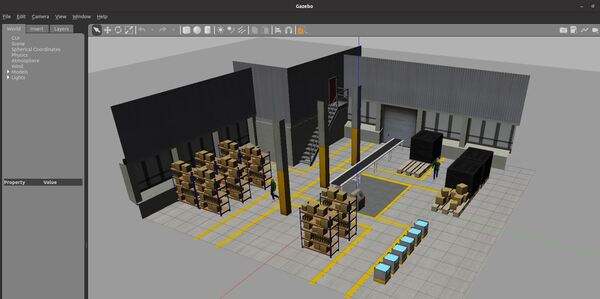
\includegraphics[width=0.8\textwidth]{warehouseEnvironment.jpg}
    \caption{The warehouse world environment [TODO better image]} \label{fig:warehouseWorld}
\end{figure}

The House world, shown in the figure \ref{fig:smallHouse}, represents a typical small, fully equipped apartment. Compared to the warehouse, this environment is significantly smaller and contains more various objects of different shapes and colors. Many of the typical household robots, like robotic vacuum cleaners, will deal with environments like this.\par

\begin{figure}[htpb]
    \centering
    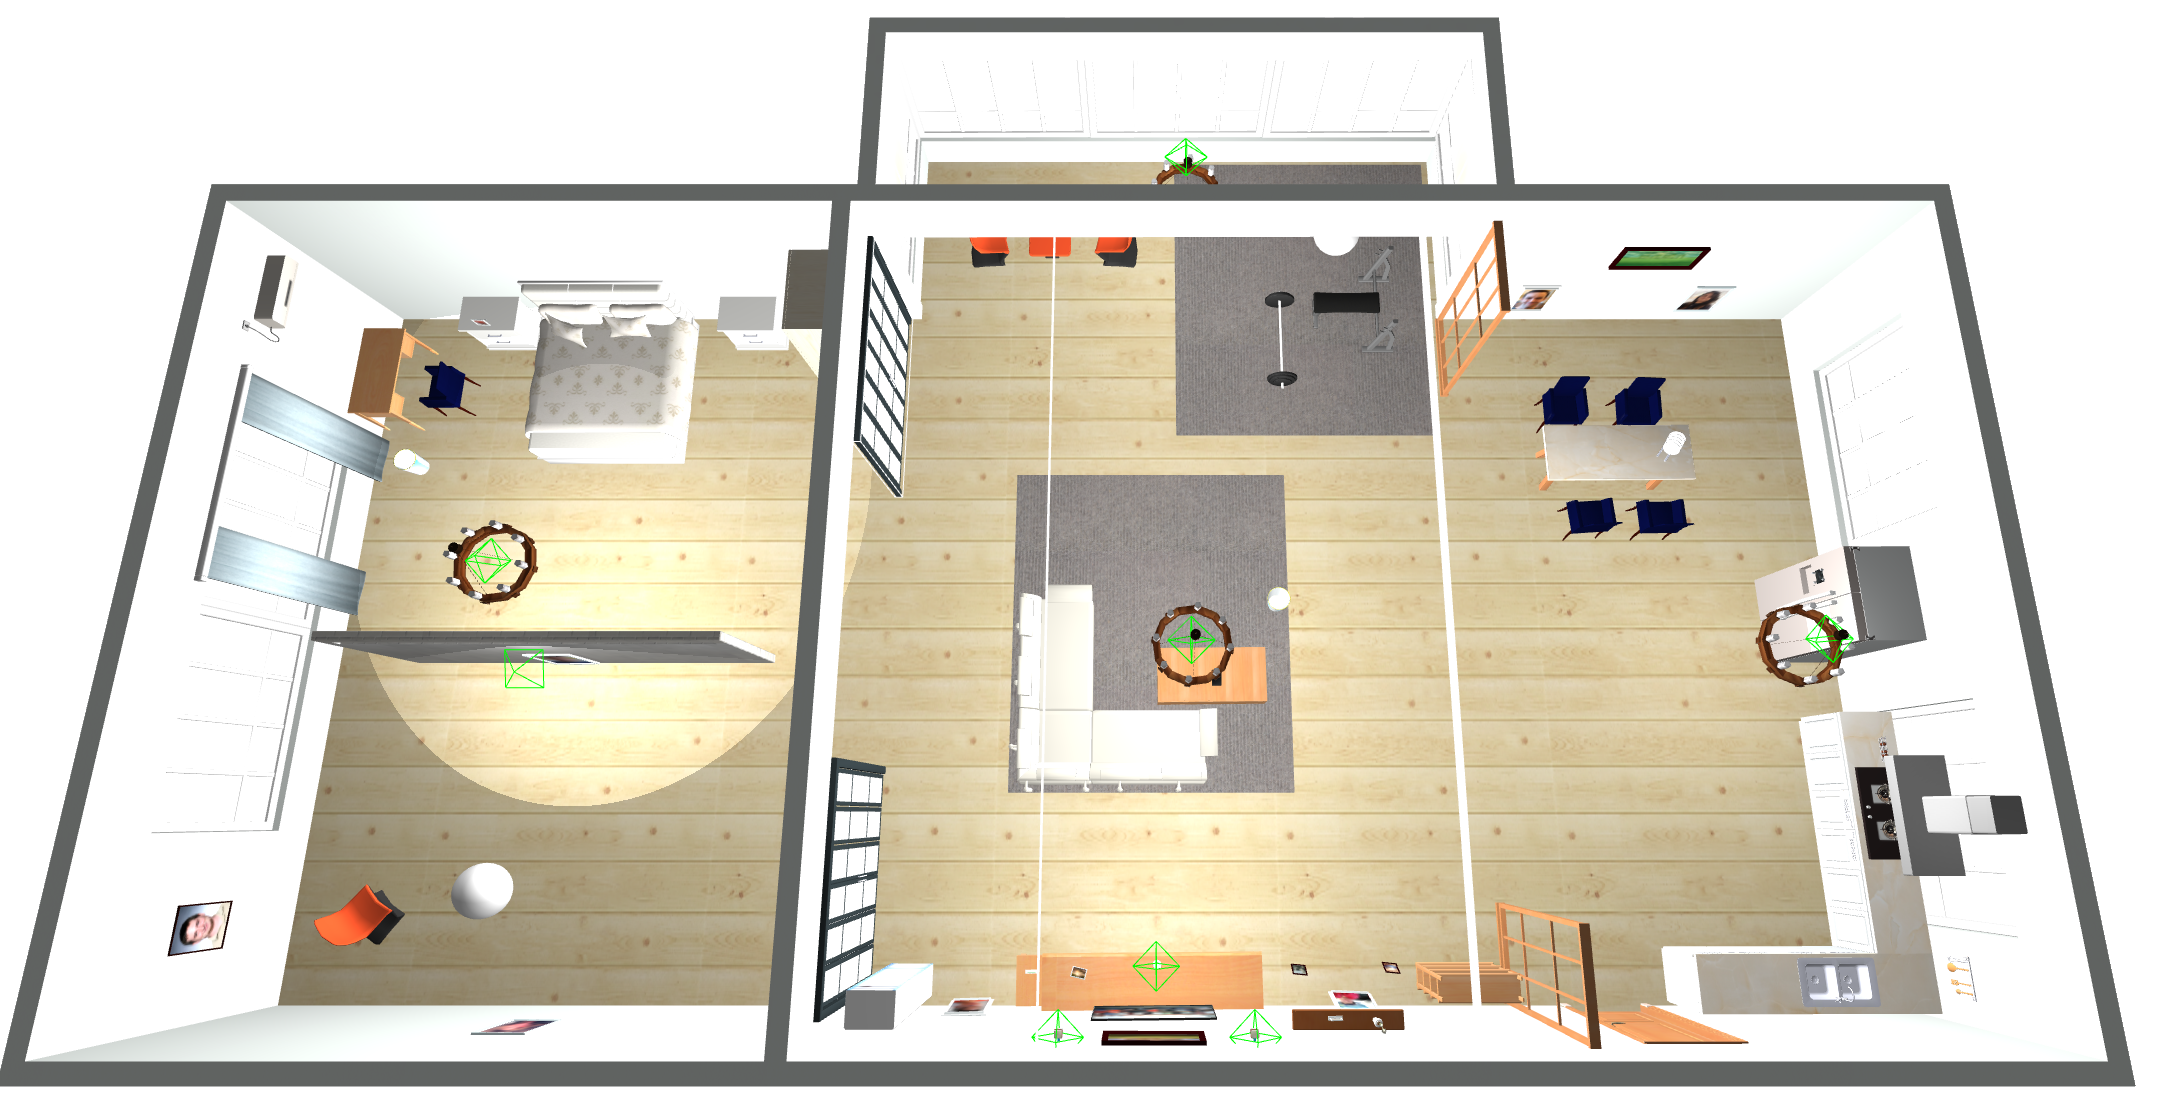
\includegraphics[width=0.8\textwidth]{smallHouse.png}
    \caption{The small house world environment [TODO ref]} \label{fig:smallHouse}
    % https://github.com/aws-robotics/aws-robomaker-small-house-world/blob/ros1/docs/images/gzweb_aws_house.png
\end{figure}

Finally, the hospital world, shown in the figure \ref{fig:hospitalWorld}, is a large, mostly empty environment from the hospital building. This environment is mostly symmetric and contains many places that look very similar, even if they are at opposite building sites. This environment was included mainly to test the algorithm's robustness against these symmetric places. Furthermore, this environment is a typical representation of any office or similar public building.\par

\begin{figure}[htpb]
    \centering
    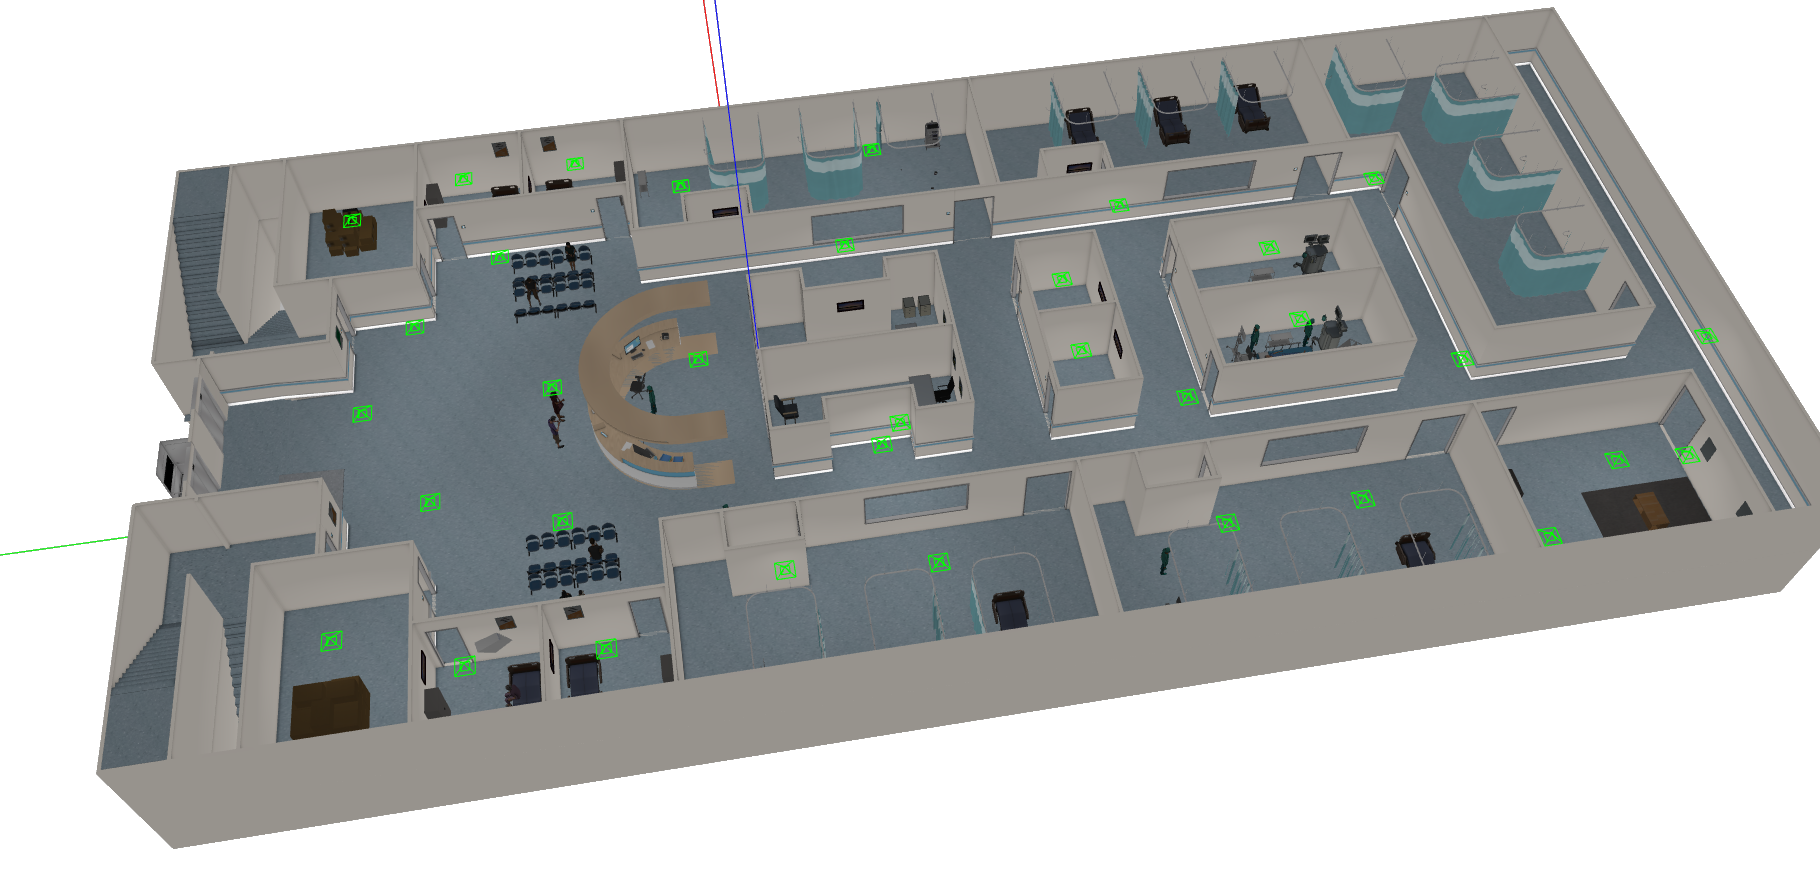
\includegraphics[width=0.8\textwidth]{Hospital.png}
    \caption{The hospital world environment [TODO ref]} \label{fig:hospitalWorld}
    % https://chowdera.com/2022/04/202204111258552961.html
\end{figure}

The algorithms were tested in each of the presented environments with several minutes long robot runs. The robot's trajectory was chosen so that the robot visits the same places several times to test the place recognition algorithm properly. All the robot runs were saved in rosbag files to ensure the repeatability of each experiment. Furthermore, every experiment for every metric presented further in this chapter has been performed on the same trajectory.\par
The dataset generated for the parameter tuning, described in the section \ref{section:parameterTuning}, and for the training of the neural networks, described in the section \ref{section:nnTraining}, were generated exclusively from the warehouse environment. The datasets' trajectory was entirely different from the trajectory used for the performance testing, but the type of the objects remained similar. In these datasets were no scenes from the other two environments.
\section{Evaluation}\label{section:Evaluation}

The result of a place recognition for a single scene can be either positive or negative. The positive evaluation means that the scene matched one of the previous ones, and the negative means that this scene is entirely new. However, in contrast to many classification algorithms, the result strongly depends on the earlier results, and the evaluation order of scenes matters. Furthermore, the classification algorithms generate the ids of the scenes instead of the direct positive/negative evaluation.\par
Let $n$ be number of scenes in the simulation and $S = \left(s_1, s_2, \dots, s_n\right)$ an ordered set of scenes that are gradually passed as an input to the algorithm. Let $P = \left(p_1, p_2, \dots, p_n\right)$ be an ordered set of the exact robot locations\footnote{$x$ and $y$ coordinates} and $O = \left(o_1, o_2, \dots, o_n\right)$ be an ordered set of exact robot orientations, on which the robot was in a time, when the appropriate scene was taken. Finally, let $R = \left(r_1, r_2, \dots, r_n \right)$ be an ordered set of scene ids, generated as an output of the place recognition algorithm.\par
Now, the result $r_i$ will be considered positive if
$$
    \exists j < i : r_j = r_i,
$$ and negative if
$$
    \forall j < i : r_j \neq r_i.
$$ The positive result is considered a false positive if the first scene with the same id is too far from the current scene in terms of location and orientation. The negative result is considered false negative if a previously saved scene is very close to the current scene in terms of location and orientation.\par
Formally, let
$$
    first\_ind(x) = \begin{cases}
        i\text{ st. } r_i = x \land \forall j < i: r_j \neq x & \text{ if $x \in R$} \\
        0                                                     & \text{ otherwise}    \\
    \end{cases}
$$
be a function that returns the index of the first scene evaluated with an id $x$. Let $r_i$ be a positive result. $r_i$ is a false positive if and only if
$$
    \| p_{first\_ind(r_i)} - p_i \| > th_\text{pos1} \lor | o_{first\_ind(r_i)} - o_i | > th_{\text{ori1}}.
$$\par
Now let $r_i$ be a negative result. $r_i$ is a false negative if and only if
$$
    \exists x < r_i:  \| p_{first\_ind(x)} - p_i \| \le th_\text{pos2} \land | o_{first\_ind(x)} - o_i | \le th_{\text{ori2}}.
$$\par
The thresholds depend on the resolution of the cell network used in the RatSLAM algorithm. Based on the robot's dimensions, the place cell size was chosen as 20 cm, slightly smaller than the robot. If the positively evaluated location is close enough, e.g., in the neighboring cells as the matched location, the algorithm still works well. Because of this, the false positive position threshold $th_\text{pos1}$ was chosen as 80 cm, which is more then four cells away. Similary, the size of orientation cells is 12°, and the false positive threshold $th_\text{pos2}$ was chosen as ca 22.9183°.\par
The false negative thresholds were chosen the same as the cell sizes, so 20 cm and 12°.

\section{System setup}\label{section:SystemSetup}

The system's performance has to be measured without influencing the program's run. This purpose serves the Node LVAnalyzer, which only subscribes to several topics and does not publish any messages. This node performs the complete performance analysis of the system.\par
This node contains a class Analyser, which performs the entire analysis. After the initialization, the class can be used by repeatedly calling its method insert. This method takes an id of a newly classified scene together with the robot's position and orientation at the scene's time. If the id is new, the position and orientation are stored, and all previously stored positions and orientations are compared to detect possible false negative. If the id already exists, the current position and orientation are compared with the stored one to detect possible false positive evaluation.\par
If the insert method is called on all scenes during the algorithm's run, the total number of true and false positives and a total number of true and false negatives is calculated. Furthermore, the analyzer generates detailed information, like ids, time, and exact positions of all false positive and negative evaluations. In addition to that, if the scene images are passed as a third optional parameter to the insert method, the Analyser will generate images of all false positive evaluations to see the difference between the wrongly matched views. This class also provides an animated live preview of all the scenes and their matches, as shown in the figure \ref{fig:analExample}.\par

\begin{figure}[htpb]
    \centering
    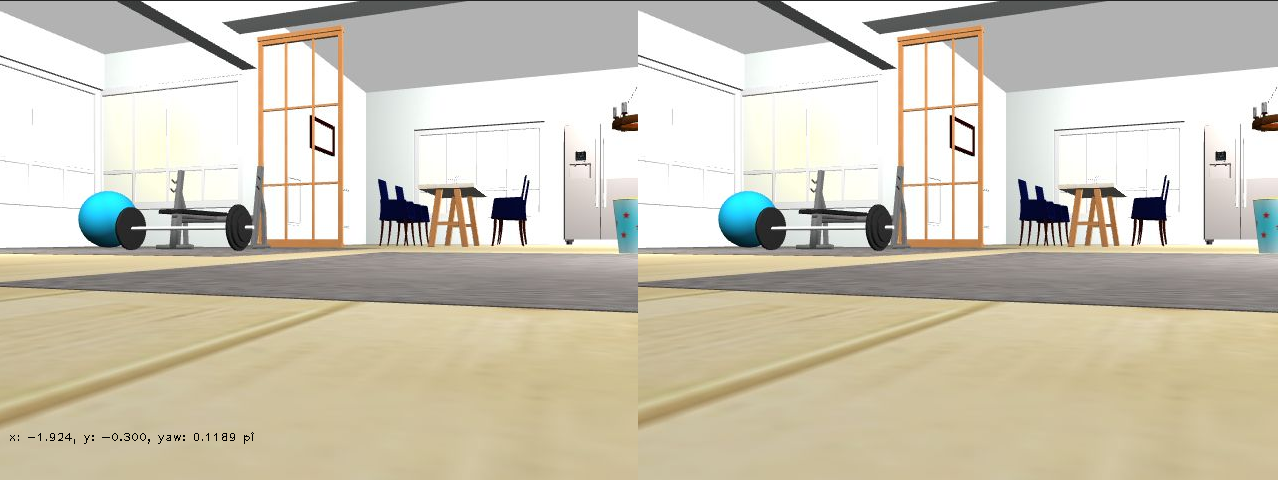
\includegraphics[width=0.8\textwidth]{analyserExample.png}
    \caption[Preview of the animation generated by the analyzer]{Preview of the animation generated by the analyzer. The left part shows a current scene and position, and the right part shows the preview of a matched scene.} \label{fig:analExample}
\end{figure}

The LVAnalyzer node is a wrapper over the Analyser class. This node subscribes to three topics, LVTemplate, Odometry, and Camera. After receiving a new matched template id from the LVTemplate topic, the exact position and scene image is found from the Odometry and Camera topics based on the timestamp of the messages. Afterward, all information is passed to the Analyser class using the insert method.

\section{Accuracy}\label{section:accuracy}

One of the essential evaluation metrics is the algorithm's accuracy, which will be measured in this section. In the beginning, the approaches presented in sections \ref{section:hierarchical} and \ref{section:2stage} will be compared using PR curves in all three environments. Afterward, the best thresholds will be picked, and the final accuracy measured for both approaches and compared with the accuracy of the visual matching used in the OpenRatSLAM.\par
The thresholds are one of the factors that influence the results the most. To find the best threshold values and to adequately compare both techniques, the accuracy, recall, and precision were measured for all possible threshold combinations with 0.01 steps. The measured values for all different thresholds were used to build the PR curves, presented in Figure \ref{fig:prCurves}.\par

\begin{figure}[!tbp]
    \centering
    \subfloat[Warehouse environment]{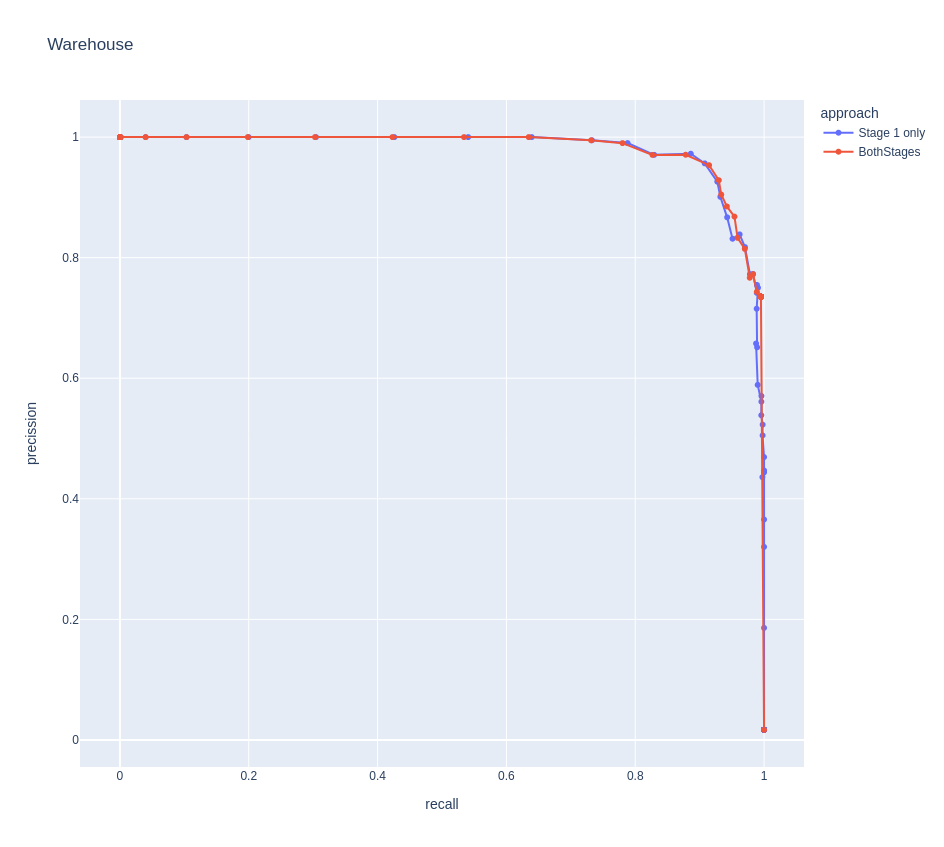
\includegraphics[height=0.3\textheight]{warehousePR.png}\label{fig:prCurvesWarehouse}}
    \hfill
    \subfloat[House environment]{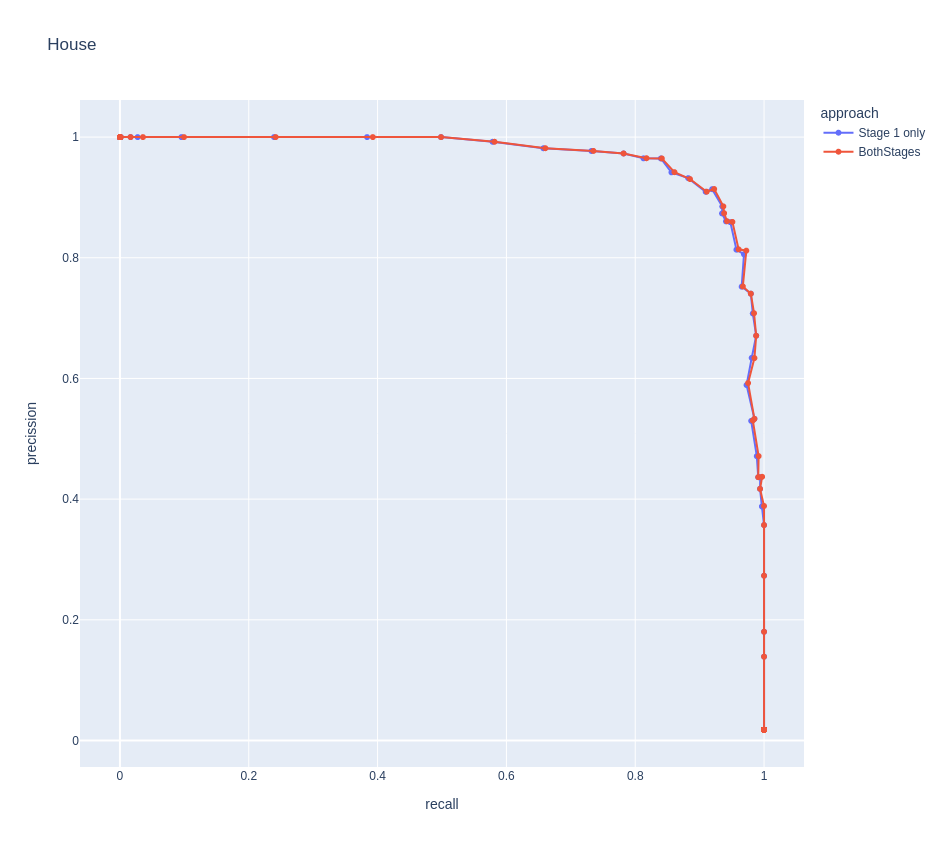
\includegraphics[height=0.3\textheight]{housePR.png}\label{fig:prCurveshouse}}
    \\
    \subfloat[Hospital environment]{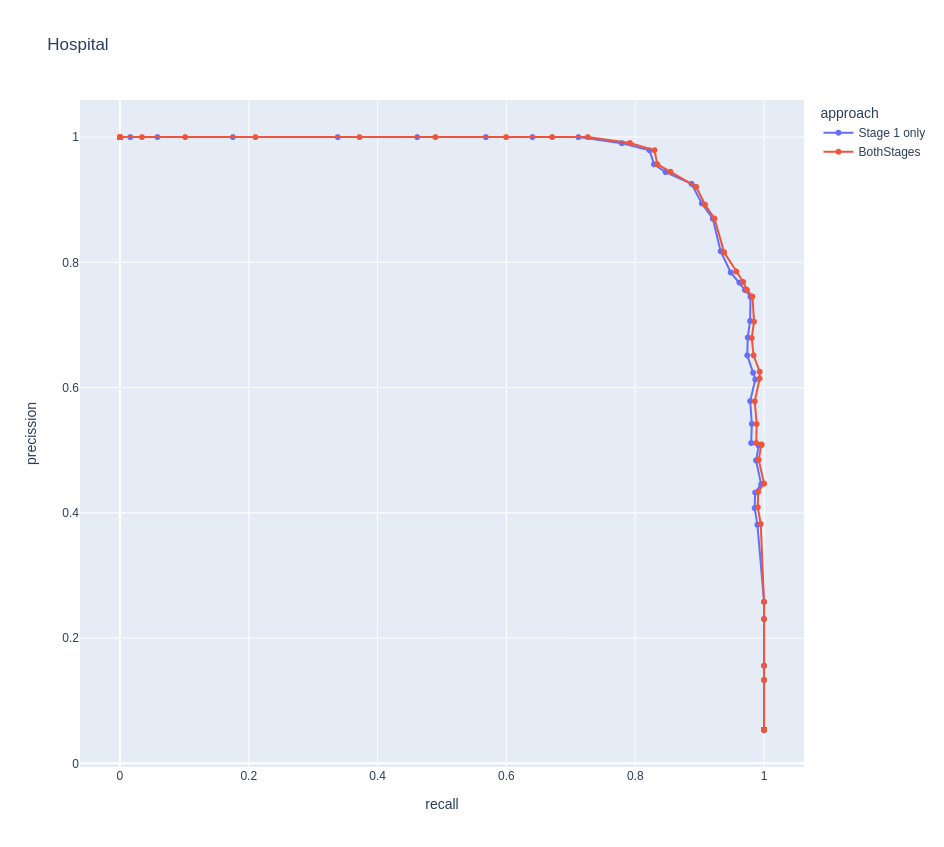
\includegraphics[height=0.3\textheight]{hospitalPR.png}\label{fig:prCurvesHospital}}
    \caption{PR Curves comparing Hierarchical and 2-Stage view matching approaches}
    \label{fig:prCurves}
\end{figure}


Because the thresholds influence only the LV matching part and not the LV building part, the local views were built and saved using the LV Dataset creator node, presented in section \ref{section:lvdatasetCreator}. This dataset was afterward used for evaluation instead of running the whole simulation, which saved a lot of time.\par
As Figure \ref{fig:prCurves} shows, both approaches have very similar results. Still, the method with two stages slightly outperforms the hierarchical approach with only the first stage by eliminating some false positive evaluations. Examples of false positives, evaluated by the first stage and eliminated by the second stage, are shown in Figure \ref{fig:eliminatedFPExamples}.\par

\begin{figure}[!tbp]
    \centering
    \subfloat{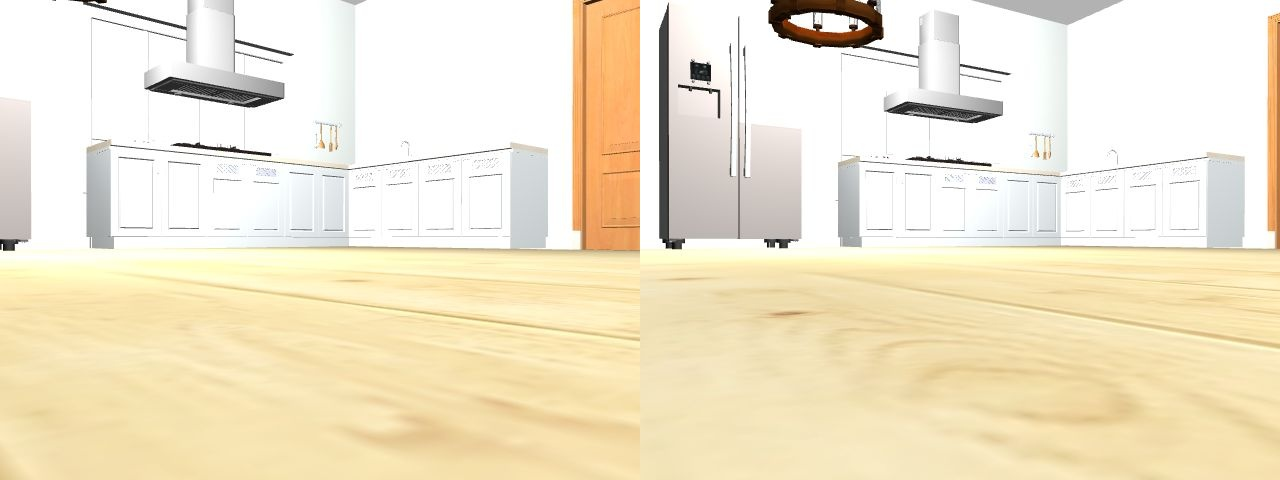
\includegraphics[width=0.8\textwidth]{eliminatedFPExample1.jpg}\label{fig:eFPEx1}}
    \\
    \subfloat{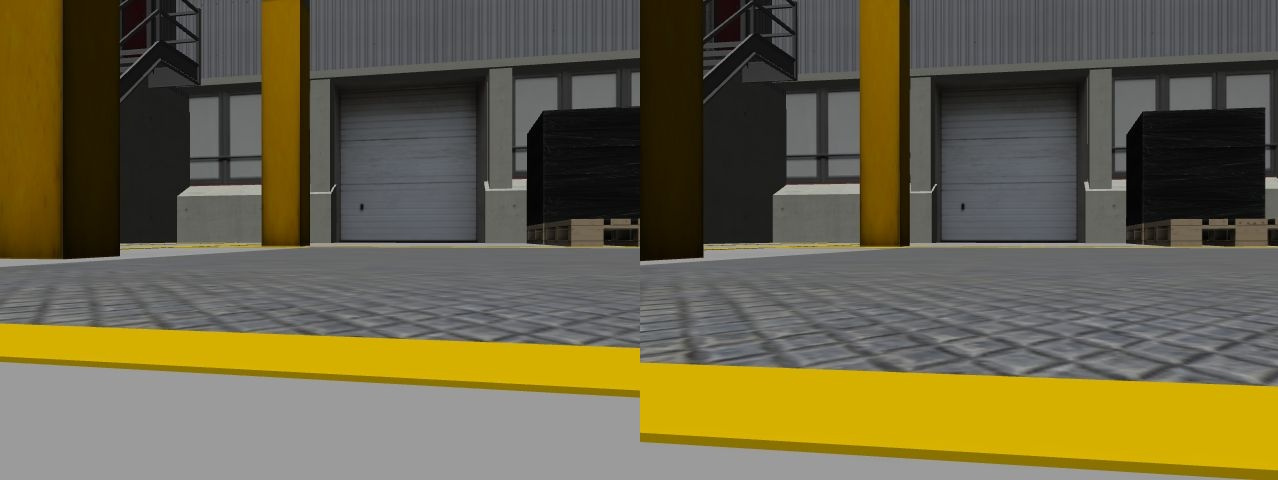
\includegraphics[width=0.8\textwidth]{eliminatedFPExample2.jpg}\label{fig:eFPEx2}}
    \caption{Examples of false positives eliminated by the second stage}
    \label{fig:eliminatedFPExamples}
\end{figure}

After the optimal thresholds were picked, the overall accuracy of both approaches was measured and compared with the accuracy of the visual place recognition used in the OpenRatSLAM. The results are shown in the table \ref{tab:accuracy}.

\begin{table}[htpb]
    \caption{Accuracy of all approaches in different environments}\label{tab:accuracy}
    \centering
    \begin{tabular}{l l l l}
        \toprule
        \textbf{}          & \textbf{1st stage only} & \textbf{both stages} & \textbf{OpenRatSLAM} \\
        \textbf{Warehouse} & 88.84 \%                & 89.28 \%             & 77.67 \%             \\
        \textbf{House}     & 86.69 \%                & 86.94 \%             & 41.25 \%             \\
        \textbf{Hospital}  & 86.19 \%                & 86.38 \%             & 79.36 \%             \\
        \bottomrule
    \end{tabular}
\end{table}

As the results show, both approaches have very similar results in all environments, but the method with both stages still slightly outperformed the technique with only the first stage. We can also see that both suggested approaches significantly outperformed the visual place recognition used in the OpenRatSLAM version in every environment, especially in the house world. Furthermore, the experiment results proved the ability to generalize on the environments diametrally different from the warehouse environment used for the model training.

\section{Average False Positive Error}\label{section:averageError}

Apart from the number of false positive and false negative evaluations, the distances of the false positives between the wrongly estimated scenes is another critical performance metric. If the false positive is close to the threshold and the distance is relatively small, then the result won't be influenced much. However, if the distance between wrongly matched scenes is very large, the negative impact on the result will be significant.\par
This section analyzes distances for every false positive result during the simulation in every environment. The exact distances for every false positive evaluation for both approaches are shown in figures \ref{fig:averageFPErrorWarehouse}, \ref{fig:averageFPErrorHouse}, and \ref{fig:averageFPErrorHospital}. The average and maximal error distance for each approach in each environment, together with the comparison with the visual place recognition used in the original RatSLAM, is shown in the table \ref{tab:averageFPError}.\par

\begin{figure}[!tbp]
    \centering
    \subfloat[1st stage only]{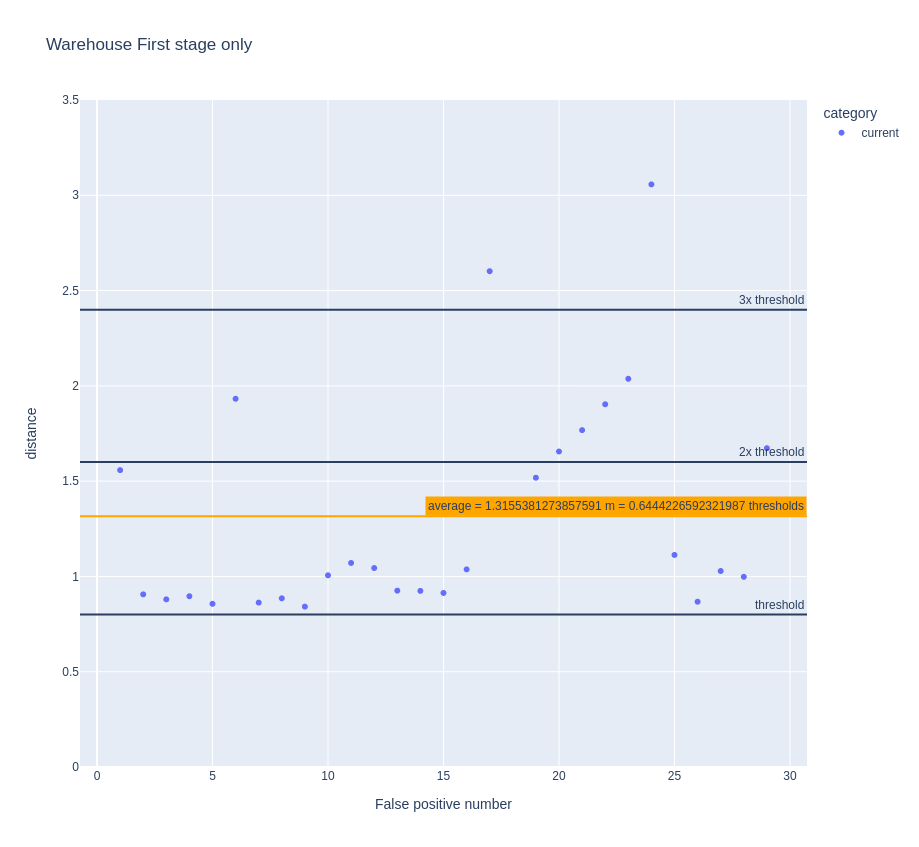
\includegraphics[width=0.5\textwidth]{warehouseFirstStageFalsePositiveDistances.png}\label{fig:FPErr11}}
    \hfill
    \subfloat[Both stages]{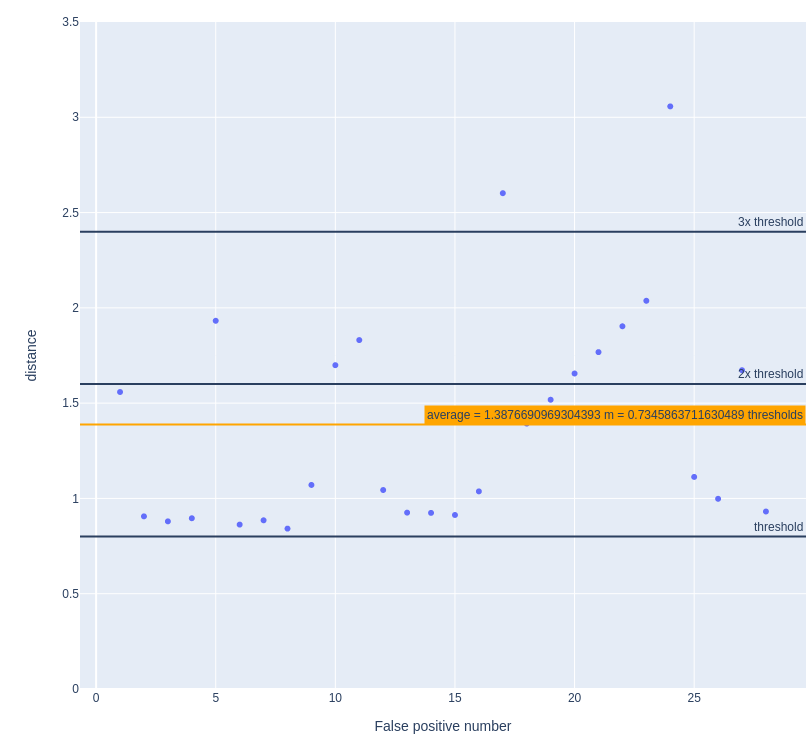
\includegraphics[width=0.5\textwidth]{warehouseBothStagesFalsePositiveDistances.png}\label{fig:FPErr12}}
    \caption{False positive distances in the warehouse environment}
    \label{fig:averageFPErrorWarehouse}
\end{figure}

\begin{figure}[!tbp]
    \centering
    \subfloat[1st stage only]{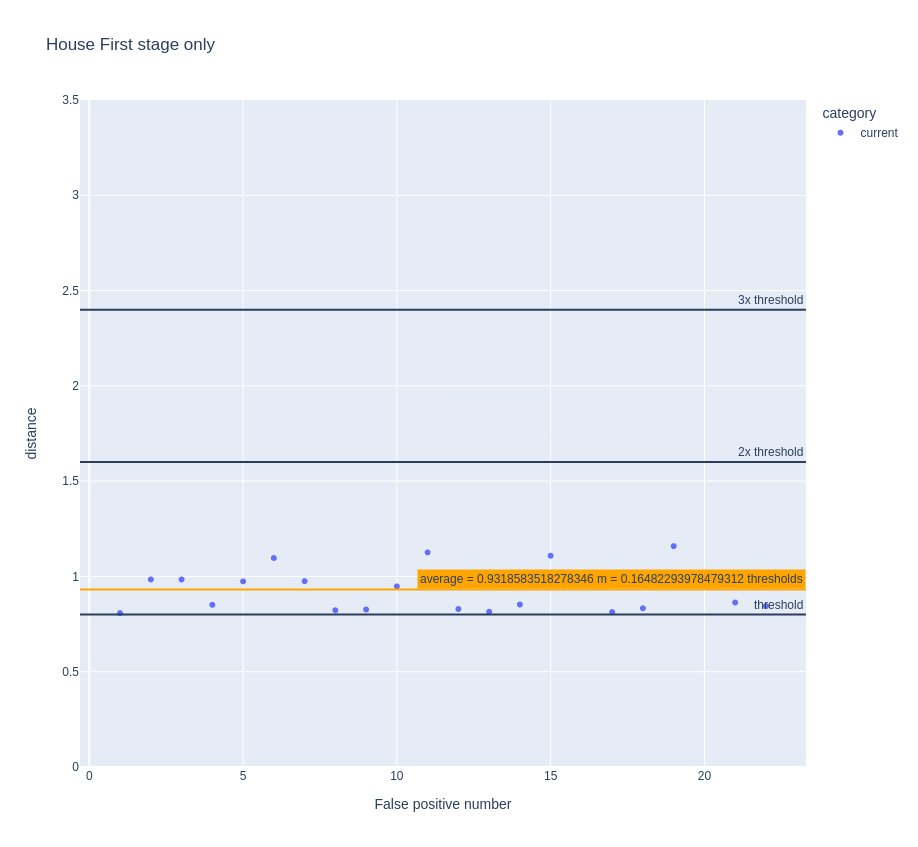
\includegraphics[width=0.5\textwidth]{houseFirstStageFalsePositiveDistances.png}\label{fig:FPErr21}}
    \hfill
    \subfloat[Both stages]{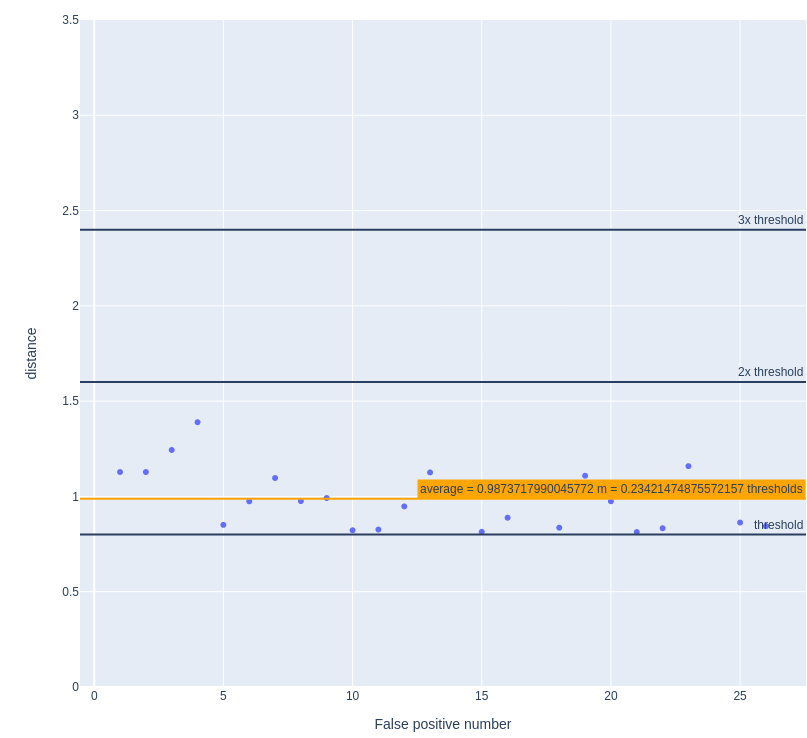
\includegraphics[width=0.5\textwidth]{houseBothStagesFalsePositiveDistances.png}\label{fig:FPErr22}}
    \caption{False positive distances in the house environment}
    \label{fig:averageFPErrorHouse}
\end{figure}

\begin{figure}[!tbp]
    \centering
    \subfloat[1st stage only]{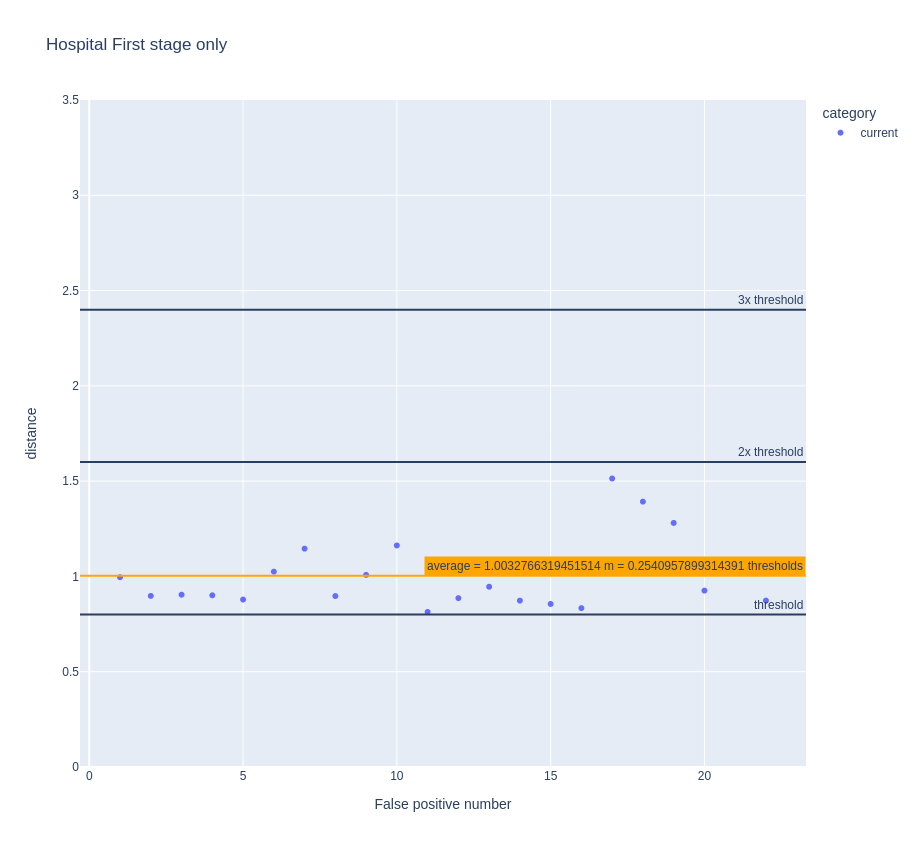
\includegraphics[width=0.5\textwidth]{hospitalFirstStageFalsePositiveDistances.png}\label{fig:FPErr31}}
    \hfill
    \subfloat[Both stages]{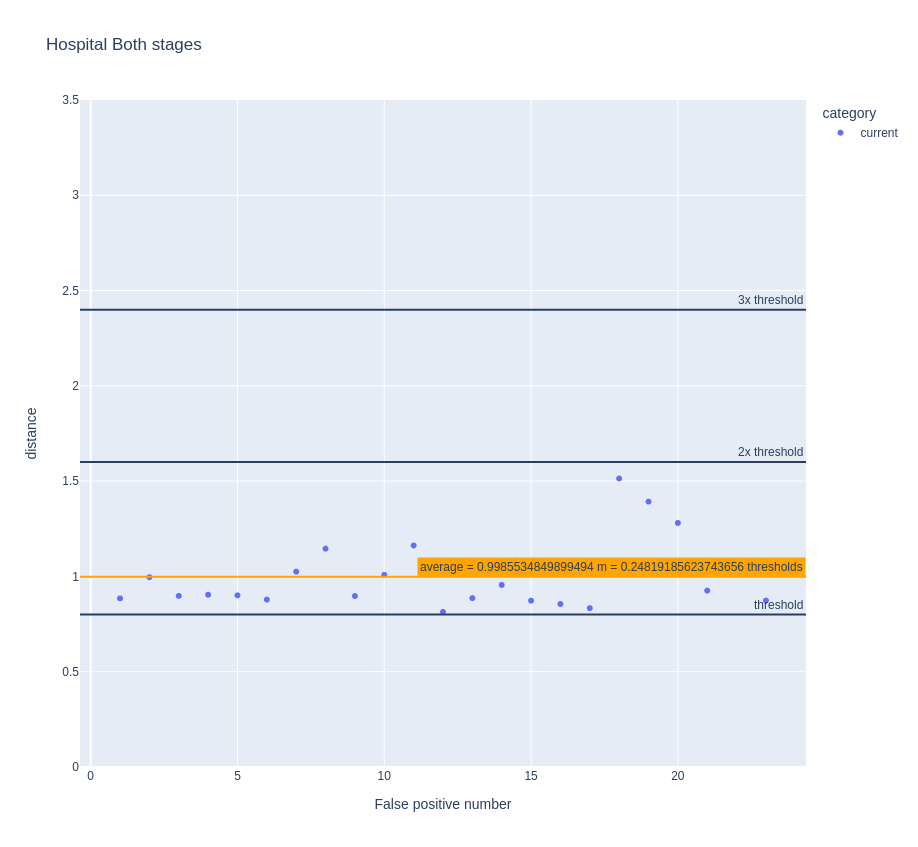
\includegraphics[width=0.5\textwidth]{hospitalBothStagesFalsePositiveDistances.png}\label{fig:FPErr32}}
    \caption{False positive distances in the hospital environment}
    \label{fig:averageFPErrorHospital}
\end{figure}

\begin{table}[htpb]
    \caption{Average and maximal errors of false positive evaluations in different environments}\label{tab:averageFPError}
    \centering
    \begin{tabular}{l | l  l| l l| l l}
        \toprule
        \textbf{}                      & \multicolumn{2}{l|}{\textbf{1st stage only}} & \multicolumn{2}{l|}{\textbf{both stages}} & \multicolumn{2}{l}{\textbf{original RatSLAM}}                             \\
        {}                             & avg                                          & max                                       & avg                                           & max    & avg    & max     \\
        \hline
        \textbf{Warehouse environment} & 1.32 m                                       & 3.06 m                                    & 1.39 m                                        & 3.06 m & 8.93 m & 11.52 m \\
        \textbf{House environment}     & 0.93 m                                       & 1.16 m                                    & 0.99 m                                        & 1.39 m & 1.84 m & 3.93 m  \\
        \textbf{Hospital environment}  & 1.00 m                                       & 1.52 m                                    & 1.00 m                                        & 1.51 m & 6.56 m & 14.57 m \\
        \bottomrule
    \end{tabular}
\end{table}

As the results show, both techniques suggested in this work showed outstanding performance in this metric. In the house and hospital environment, the average error lies only 13-20 cm away from the threshold, which is less than 25 \% of the threshold size. Moreover, all evaluated false negatives in these environments are not farther than twice the threshold from the matched scene. This means that all wrongly evaluated matches are still very close to the threshold and shouldn't cause almost any damage to the final result. Some errors in the warehouse environment were slightly larger, but they were only exceptional cases, and most of the wrongly classified matches are still very close to the threshold.\par
On the other hand, the results of the visual place recognition used in the original RatSLAM were significantly worse. As the results suggest, most of the wrongly evaluated scenes were spread over the whole environment, and the distances between the incorrectly matched scenes were huge. The most significant errors can be observed in the hospital environment, which drastically influenced the generated experience map, as discussed in the section \ref{section:RatSalmIntegration}.\par
According to this metric, both presented approaches significantly outperformed the visual place recognition used in the original RatSLAM.

\section{Time Performance}\label{section:timePerformance}

Another important property is the time of the local view template building and especially the time of comparing two templates. The time of the template building and comparing the two templates are measured separately. The reason is that the template building is done only once per scene, independently of the length of the algorithm's run. However, comparing the two templates is done more times for every scene. Namely, every new scene is compared with all previously saved scenes whose number increases over time, especially in large and various environments. Therefore, the time of the matching is the critical part and must be as fast as possible. In contrast, the time of the building can be significantly larger as long as it stays smaller than the period between two sensor inputs.\par
The system was tested on a Laptop with the following parameters:

\begin{description}[labelwidth=5em,leftmargin =\dimexpr\labelwidth+\labelsep\relax]
    \item[\textbf{Processor}:] Intel${}^{\text{\tiny{\textregistered}}}$ Core™ i7-8650U Processor (1.9 - 4.2 GHz) \footnote{\tiny{\url{https://ark.intel.com/content/www/us/en/ark/products/124968/intel-core-i7-8650u-processor-8m-cache-up-to-4-20-ghz.html}}}
    \item[\textbf{RAM}:]
          \begin{itemize}
              \item 4 GiB Row of chips DDR4 Synchronous Unbuffered (Unregistered) 2400 MHz (0,4 ns)
              \item 8 GiB SODIMM DDR4 Synchronous Unbuffered (Unregistered) 2400 MHz (0,4 ns)
          \end{itemize}
    \item[\textbf{OS}:] Kubuntu 21.10 x86\_64,
\end{description}

inside of the virtual machine, with the following limitations and operating system:

\begin{description}[labelwidth=5em]
    \item[\textbf{RAM}:] 8 GiB
    \item[\textbf{OS}:] Ubuntu 20.04 LTS x86\_64.
\end{description}

The GPU did not have CUDA support, so all the computations were performed on a CPU.\par
Figures \ref{fig:timesWarehouse}, \ref{fig:timesHouse}, and \ref{fig:timesHospital} show the LV building times for each scene and also matching times for each pair of compared scenes in all the environments. The table \ref{tab:averageTimes} shows the average times for each approach in every environment compared with the visual place recognition used in the OpenRatSLAM.


\begin{figure}[!tbp]
    \centering
    \subfloat[LV building times]{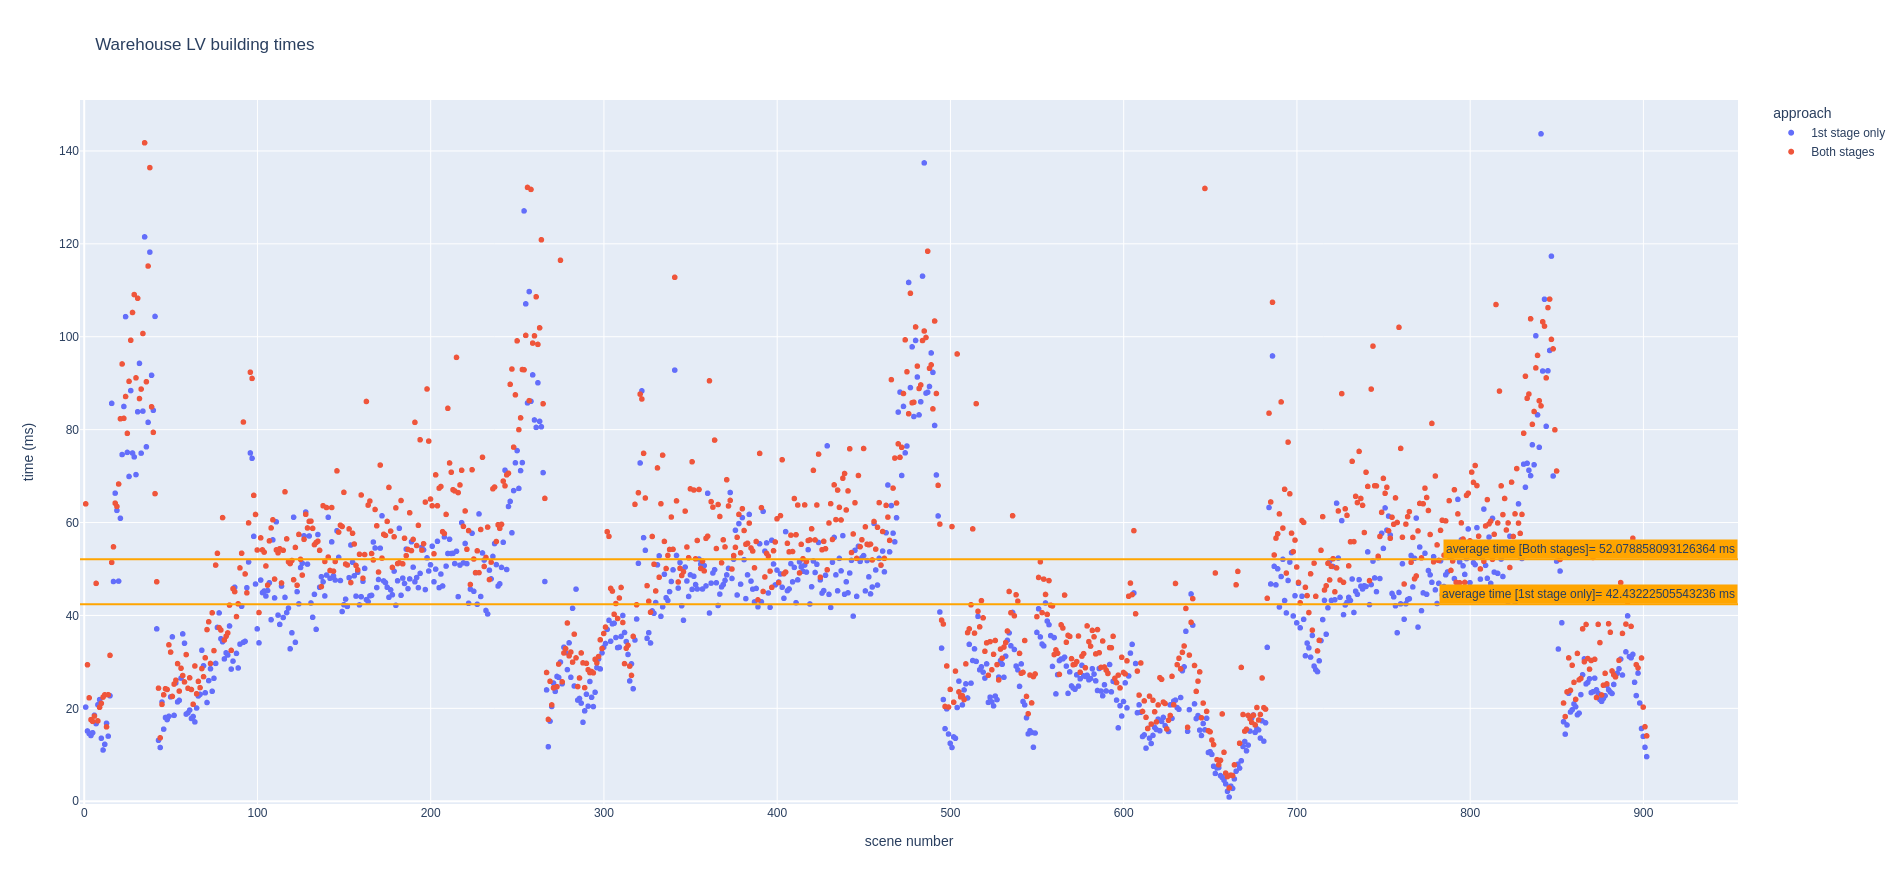
\includegraphics[width=0.8\textwidth]{warehouseBuildingTimes.png}\label{fig:timesWH1}}
    \\
    \subfloat[LV matching times]{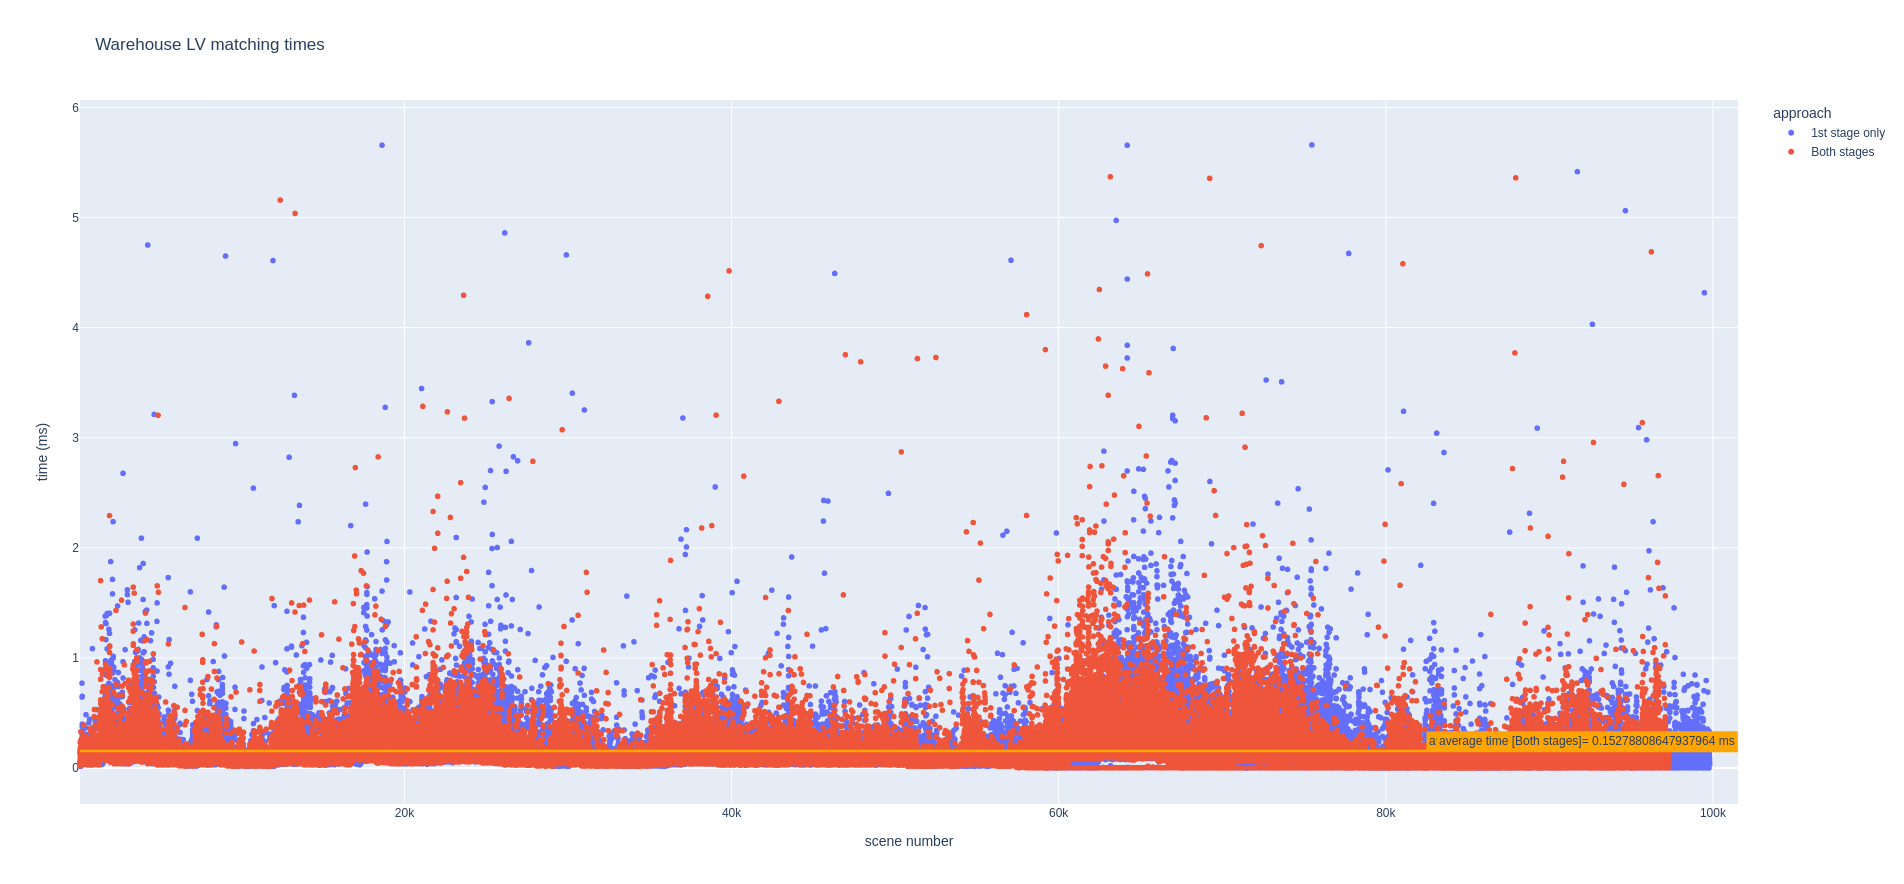
\includegraphics[width=0.8\textwidth]{warehouseMatchingTimes.png}\label{fig:timesWH2}}
    \caption{Computation times in the warehouse environment}
    \label{fig:timesWarehouse}
\end{figure}

\begin{figure}[!tbp]
    \centering
    \subfloat[LV building times]{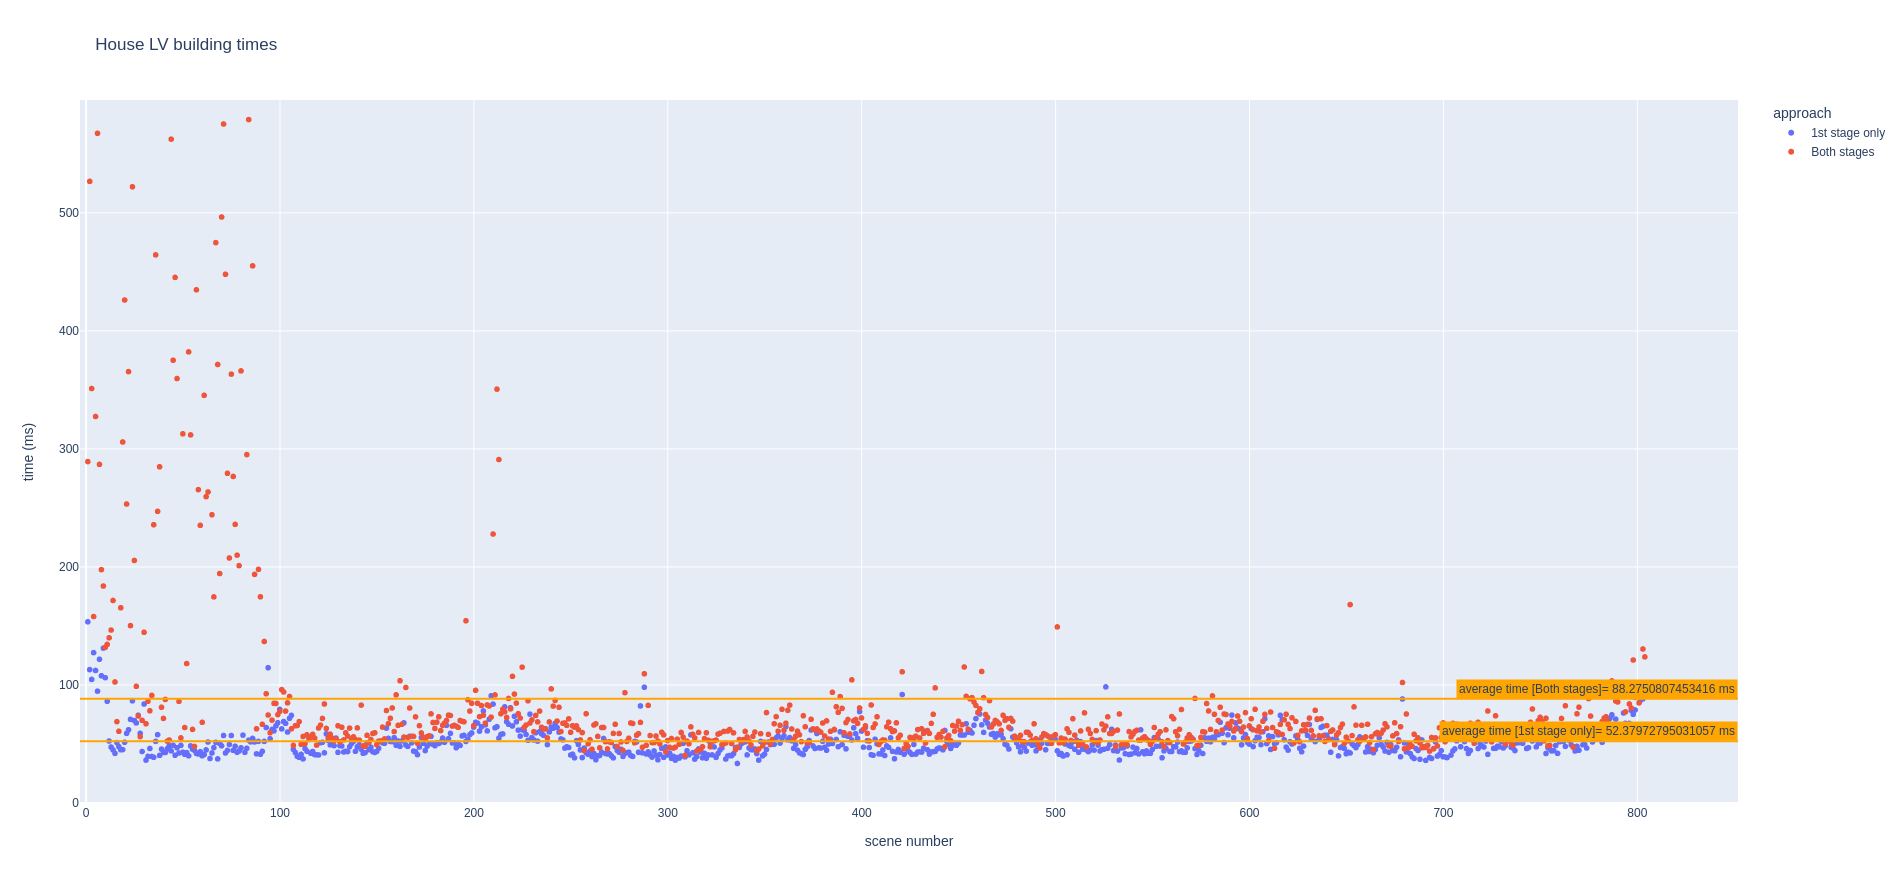
\includegraphics[width=0.8\textwidth]{houseBuildingTimes.png}\label{fig:timesHS1}}
    \\
    \subfloat[LV matching times]{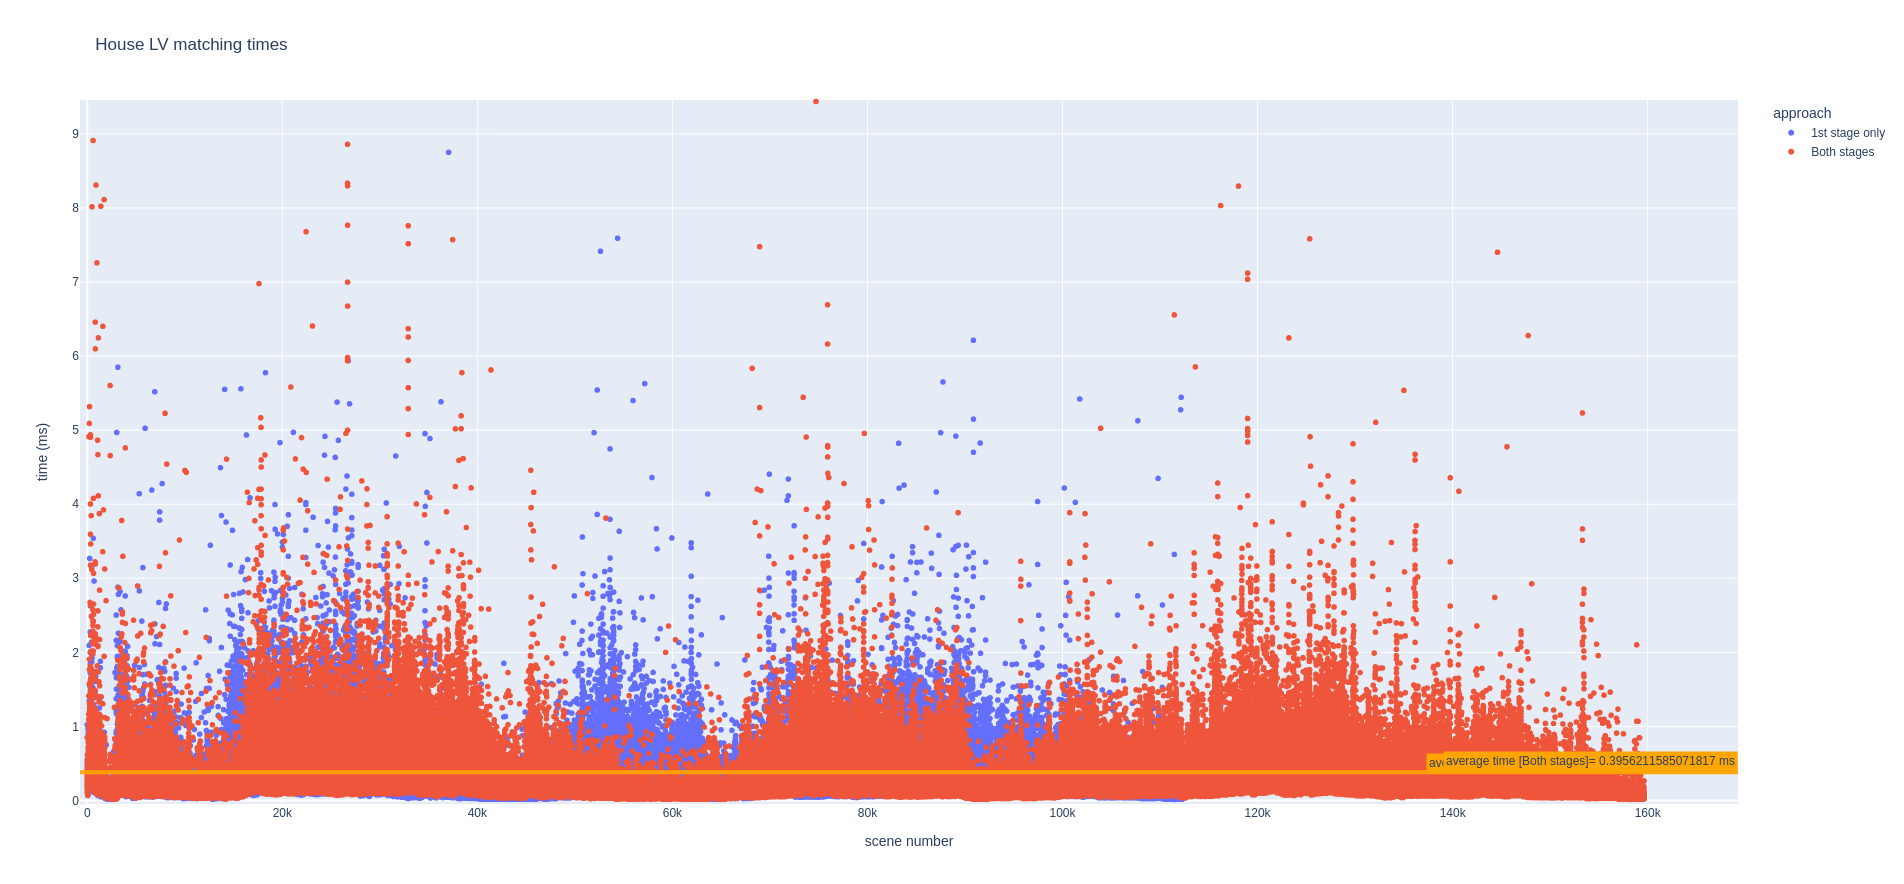
\includegraphics[width=0.8\textwidth]{houseMatchingTimes.png}\label{fig:timesHS2}}
    \caption{Computation times in the house environment}
    \label{fig:timesHouse}
\end{figure}

\begin{figure}[!tbp]
    \centering
    \subfloat[LV building times]{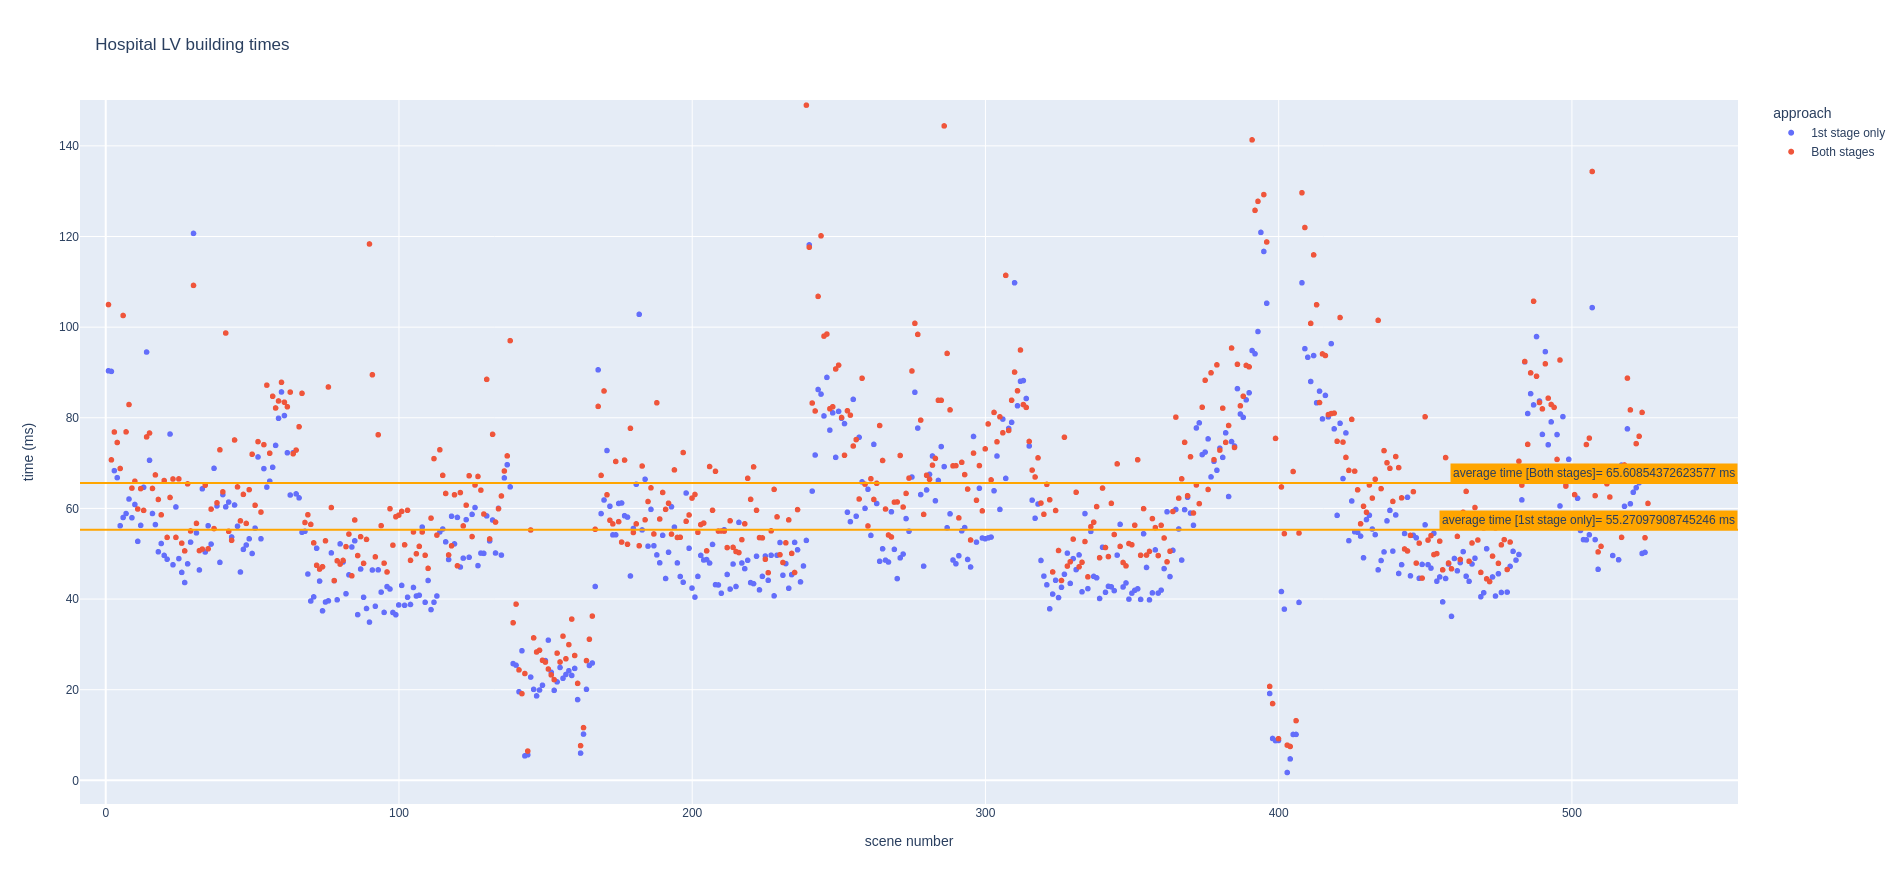
\includegraphics[width=0.8\textwidth]{hospitalBuildingTimes.png}\label{fig:timesHO1}}
    \\
    \subfloat[LV matching times]{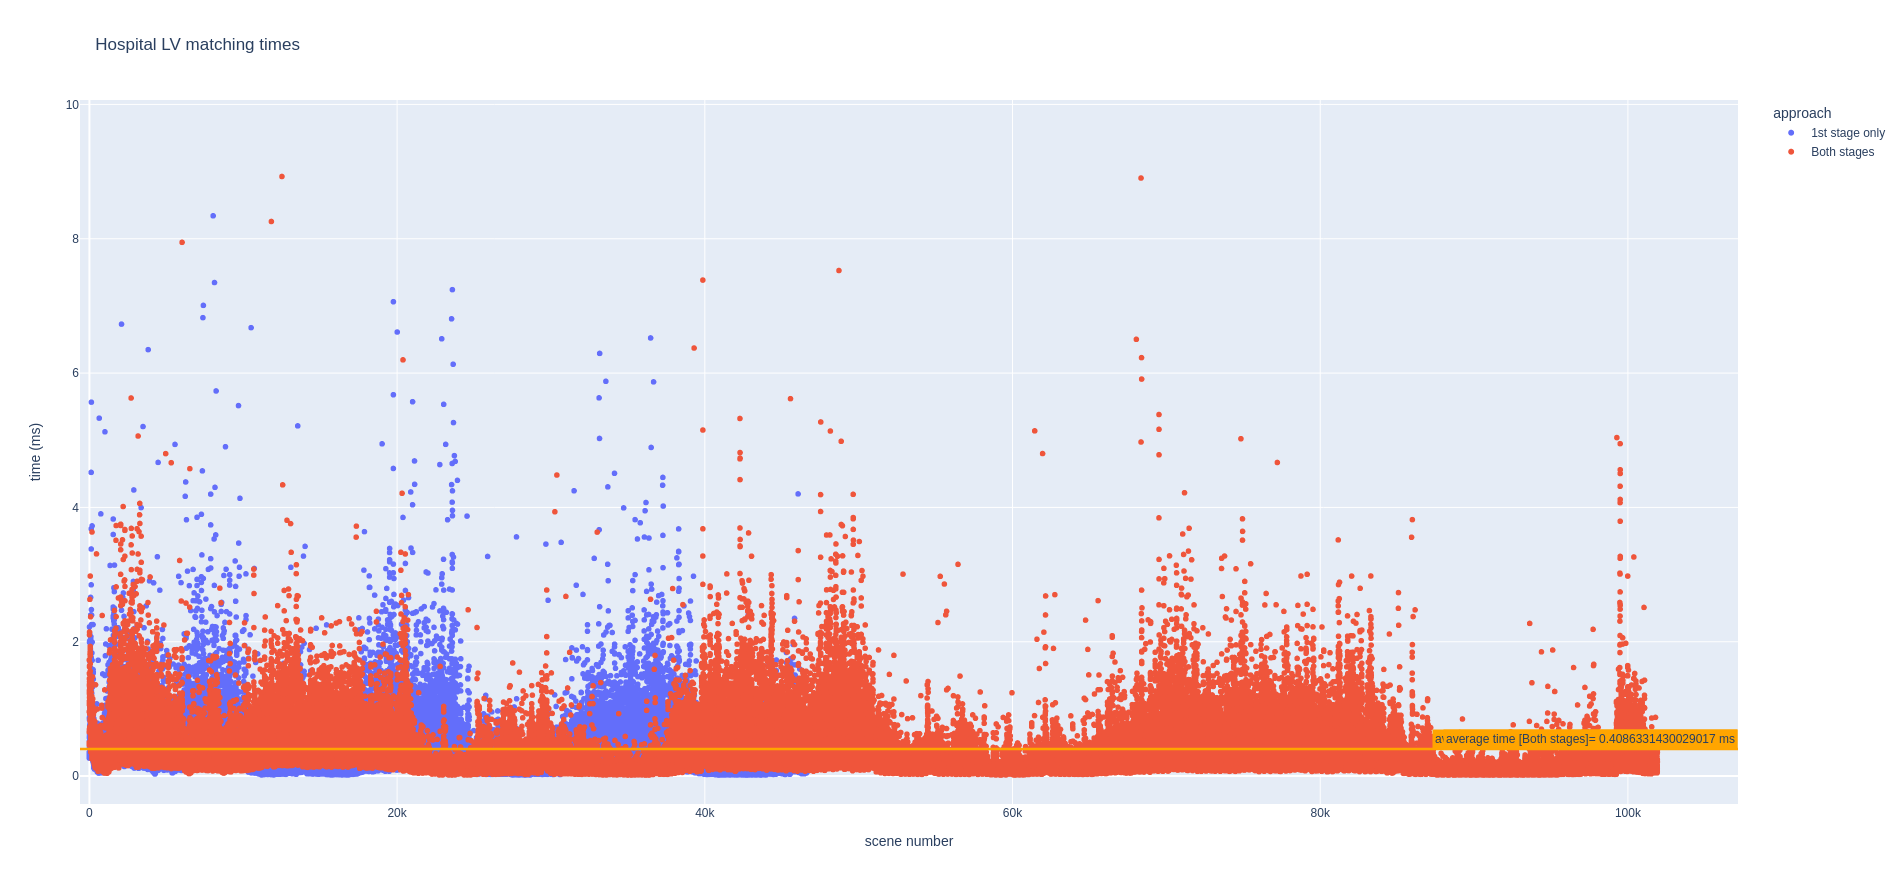
\includegraphics[width=0.8\textwidth]{hospitalMatchingTimes.png}\label{fig:timesHO2}}
    \caption{Computation times in the hospital environment}
    \label{fig:timesHospital}
\end{figure}

\begin{table}[htpb]
    \caption{Average times of LV matching and building in the different environments}\label{tab:averageTimes}
    \centering
    \begin{tabular}{l | l  l| l l| l l}
        \toprule
        \textbf{}          & \multicolumn{2}{l|}{\textbf{1st stage only}} & \multicolumn{2}{l|}{\textbf{both stages}} & \multicolumn{2}{l}{\textbf{OpenRatSLAM}}                                  \\
        {}                 & build                                        & match                                     & build                                    & match    & build    & match    \\
        \hline
        \textbf{Warehouse} & 42.432 ms                                    & 0.153 ms                                  & 52.078 ms                                & 0.159 ms & 2.053 ms & 0.083 ms \\
        \textbf{House}     & 52.380 ms                                    & 0.396 ms                                  & 88.265 ms                                & 0.368 ms & 1.448 ms & 0.137 ms \\
        \textbf{Hospital}  & 55.271 ms                                    & 0.399 ms                                  & 65.609 ms                                & 0.409 ms & 1.762 ms & 0.092 ms \\
        \bottomrule
    \end{tabular}
\end{table}

The table and graphs show that the approach that uses only the first stage can build the local views considerably faster than the 2-stage approach. The time difference is caused by the feature extraction, which is present only in the 2-stage approach. However, the time difference is not so significant. Most importantly, the techniques are significantly faster than the frequency of the sensors, so the time performance of local view building of both methods is satisfactory. As we can see, the LV building is significantly slower than the LV building in the OpenRatSLAM. However, the OpenRatSLAM works with sensors with significantly higher frequency\footnote{In the experiments, the frequency of the camera was 15 times higher than frequency of the LiDAR.}, so the LV building is done significantly more often, and the total resources consumption of the LV building process is comparable with the total consumption of the approaches presented in this work.\par
The times of the view matching of both approaches are almost the same, so the overhead caused by feature comparison in the second stage is practically negligible. Even if the times are circa 2 to 4 times larger than the times measured by the OpenRatSLAM, the number of saved views is significantly smaller, as shown in table \ref{tab:memory}, so the total comparison time for each scene will be at the end smaller than in the OpenRatSLAM approach. Furthermore, the times are significantly smaller than 1 ms, so there could be saved up to a thousand different local views to compare until the total comparison time reaches the sensors period. This means that this approach will also be suitable for very long time runs in huge environments.

\section{Memory Consumption}\label{section:memoryConsumption}

Especially for the robots with low-performant controllers, for example, older Raspberry PI, RAM is a very limited resource, so the memory needed for storing the local views needs to be as small as possible. Therefore another metric evaluated in the algorithms is the consumption of the memory. The measurement results are shown in the table \ref{tab:memory}.\par

\begin{table}[htpb]
    \caption{Average memory consumption of the algorithms in the different environments}\label{tab:memory}
    \centering
    \begin{tabular}{l | l  l| l l| l l}
        \toprule
        \textbf{}          & \multicolumn{2}{l|}{\textbf{1st stage only}} & \multicolumn{2}{l|}{\textbf{both stages}} & \multicolumn{2}{l}{\textbf{original RatSLAM}}                                                             \\
        {}                 & $\oslash$ LV size                            & $\oslash$ LVs stored                      & $\oslash$ LV size                             & $\oslash$ LVs st. & $\oslash$ LV size & $\oslash$ LVs st. \\
        \hline
        \textbf{Warehouse} & 78 B                                         & 194                                       & 1102 B                                        & 191               & 600 B             & 312               \\
        \textbf{House}     & 128 B                                        & 219                                       & 1152 B                                        & 216               & 600 B             & 445               \\
        \textbf{Hospital}  & 130 B                                        & 151                                       & 1154 B                                        & 148               & 600 B             & 219               \\
        \bottomrule
    \end{tabular}
\end{table}

The original RatSLAM uses a compressed 60x10 pixels big grayscale image as a local view template, so the memory needed for storing a single local view is always constant. However, the memory required for storing a single LV in the approaches suggested in this work differs for each local view and depends on the number of clusters detected by the DBScan algorithm. The difference between the size of the LV templates used in the approach with only the first stage and with both stages differs by a feature vector of 256 floating point numbers. Therefore, as follows from the table, the memory consumption of the first stage-only approach is significantly smaller than while also using the second stage.\par
The memory needed for storing the local views using the 2-stage approach is, on average, almost twice as large as the memory required for storing the lv template in the original RatSLAM approach. However, the number of stored templates in the original RatSLAM is almost twice larger than the number of stored templates in the 2-stage approach, so the total memory consumption remains similar. More interesting is the algorithm with only the first stage, in which a single local view consumes about six times less memory than the original RatSLAM approach. Furthermore, this approach stored, on average, significantly fewer local views than the original RatSLAM algorithm, so the total memory consumption is up to 12 times lower than in the original RatSLAM.

\section{RatSLAM Integration}\label{section:RatSalmIntegration}

The last metric to test is the integration with the RatSLAM. This section will integrate the scene recognition algorithm with the RatSLAM ROS system, generating the final experience maps. Finally, the maps generated for both approaches will be compared with the exact trajectory generated by the simulator and the experience map generated by the OpenRatSLAM with only visual scene recognition.\par
Even if the other evaluation techniques proved the significantly better performance of the methods suggested in this work, it is unclear if they will produce satisfactory results in connection with the RatSLAM, primarily because of the significantly lower frequency of the sensors. Therefore, this section aims to show that the improved performance compensates for the frequency loss of the sensors and that the generated results are at least as good as the results produced by the OpenRatSLAM or even better.\par

\begin{figure}[!tbp]
    \centering
    \subfloat[1st Stage only approaches]{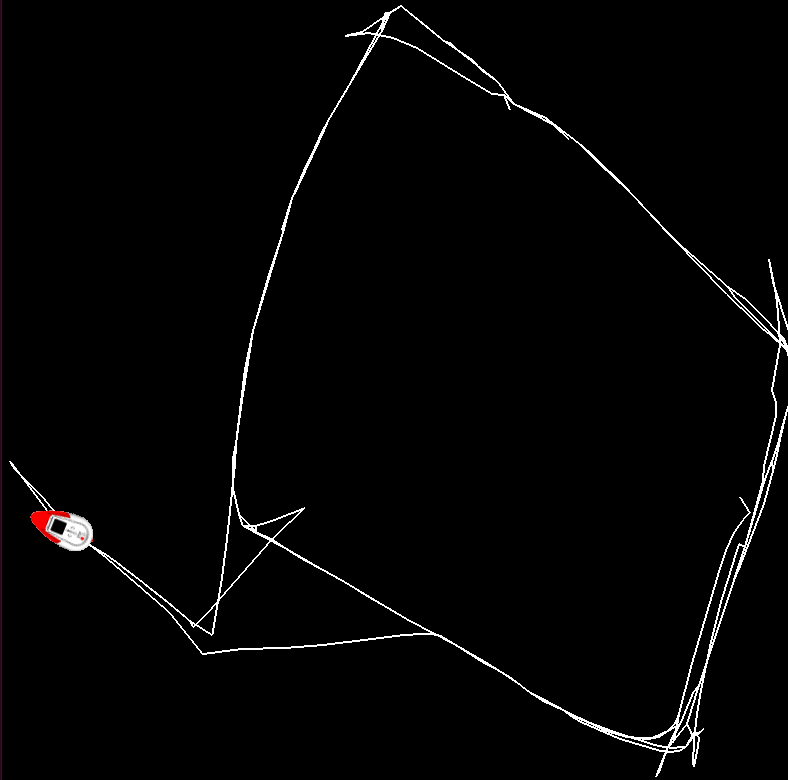
\includegraphics[height=0.3\textheight]{warehouse-1stStage.png}\label{fig:mapsWarehouse1st}}
    \hfill
    \subfloat[Both stages approaches]{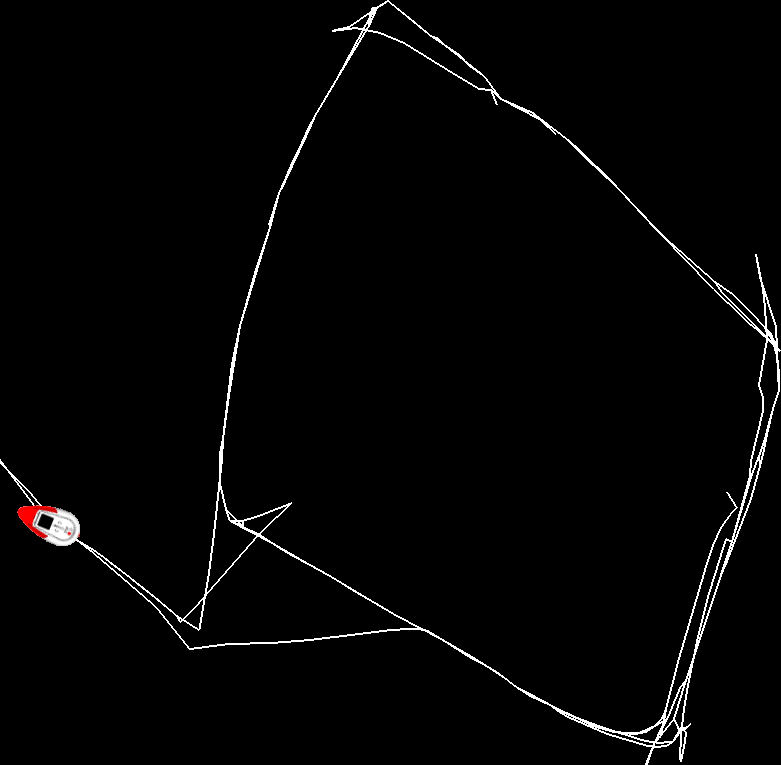
\includegraphics[height=0.3\textheight]{warehouse-bothStages.png}\label{fig:mapsWarehouseBot}}
    \\
    \subfloat[OpenRatSLAM]{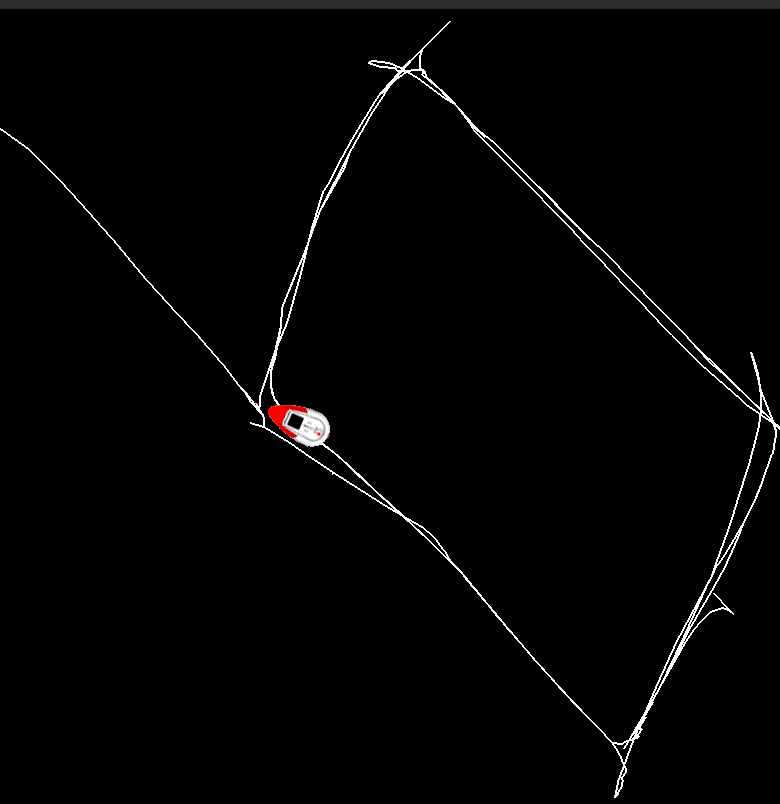
\includegraphics[height=0.3\textheight]{warehouse-ratslam.png}\label{fig:mapsWarehouseRat}}
    \hfill
    \subfloat[Exact trajectory]{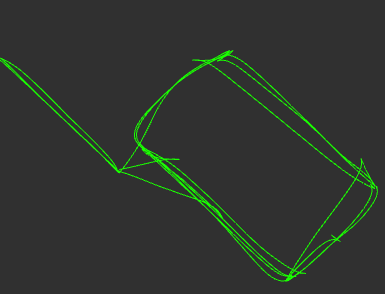
\includegraphics[height=0.3\textheight]{warehouse-exact.png}\label{fig:mapsWarehouseEx}}
    \caption{Generated experience maps in the warehouse environment}
    \label{fig:mapsWarehouse}
\end{figure}

\begin{figure}[!tbp]
    \centering
    \subfloat[1st Stage only approaches]{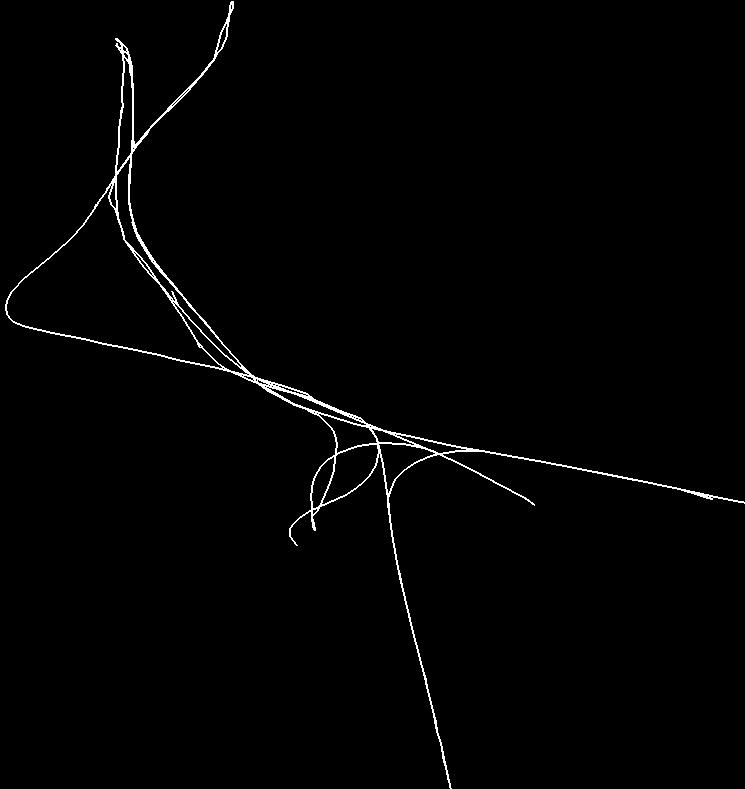
\includegraphics[height=0.3\textheight]{house-1stStage.png}\label{fig:mapsHouse1st}}
    \hfill
    \subfloat[Both stages approaches]{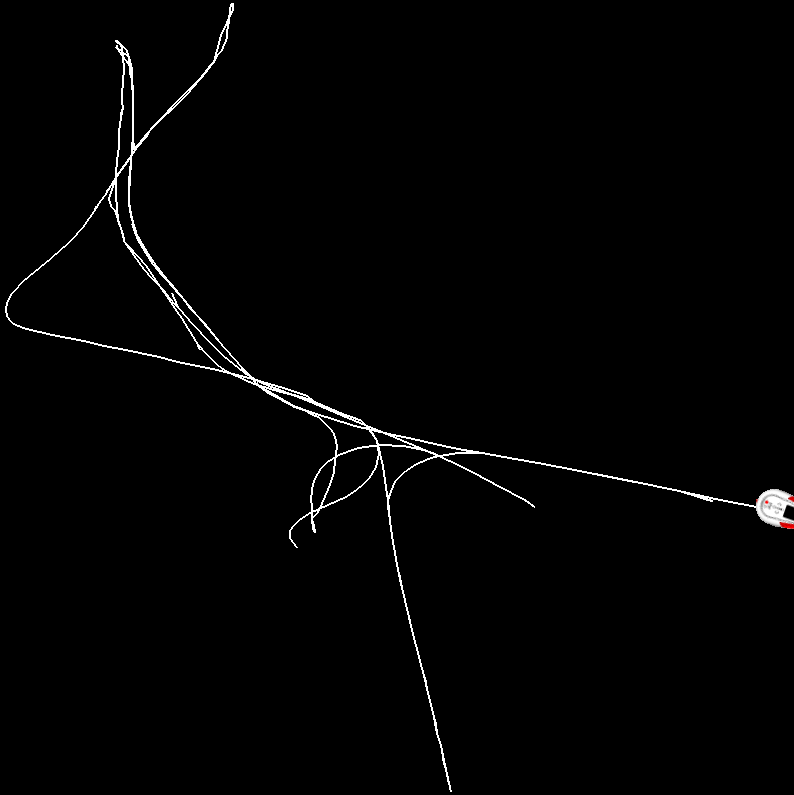
\includegraphics[height=0.3\textheight]{house-bothStages.png}\label{fig:mapsHouseBot}}
    \\
    \subfloat[OpenRatSLAM]{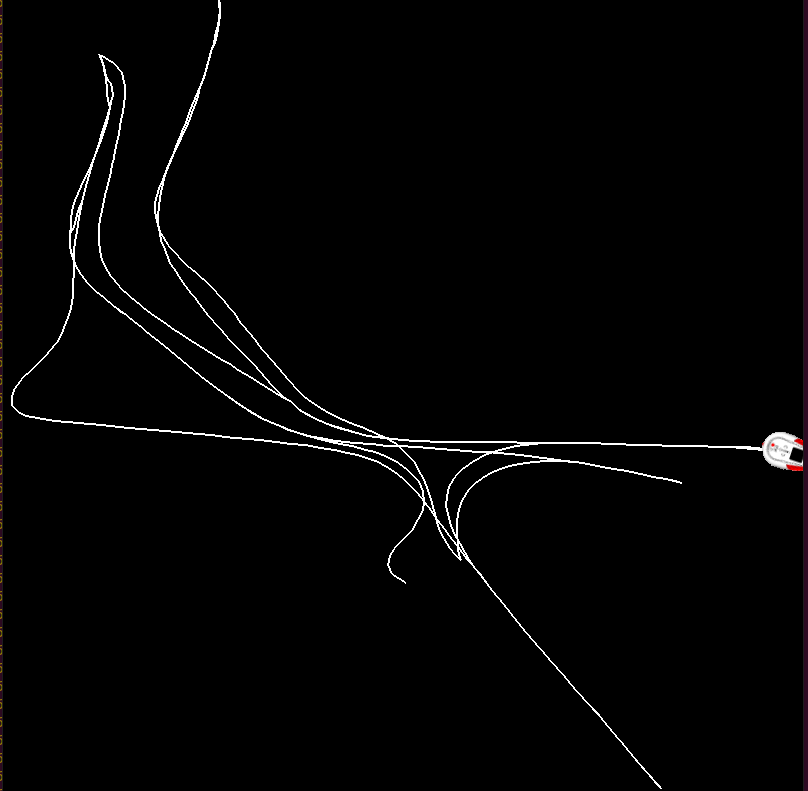
\includegraphics[height=0.3\textheight]{house-ratslam.png}\label{fig:mapsHouseRat}}
    \hfill
    \subfloat[Exact trajectory]{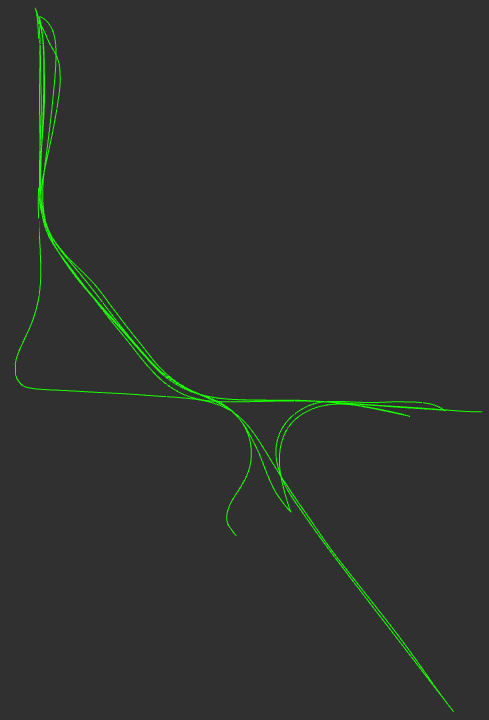
\includegraphics[height=0.3\textheight]{house-exact.png}\label{fig:mapsHouseEx}}
    \caption{Generated experience maps in the house environment}
    \label{fig:mapsHouse}
\end{figure}

\begin{figure}[!tbp]
    \centering
    \subfloat[1st Stage only approaches]{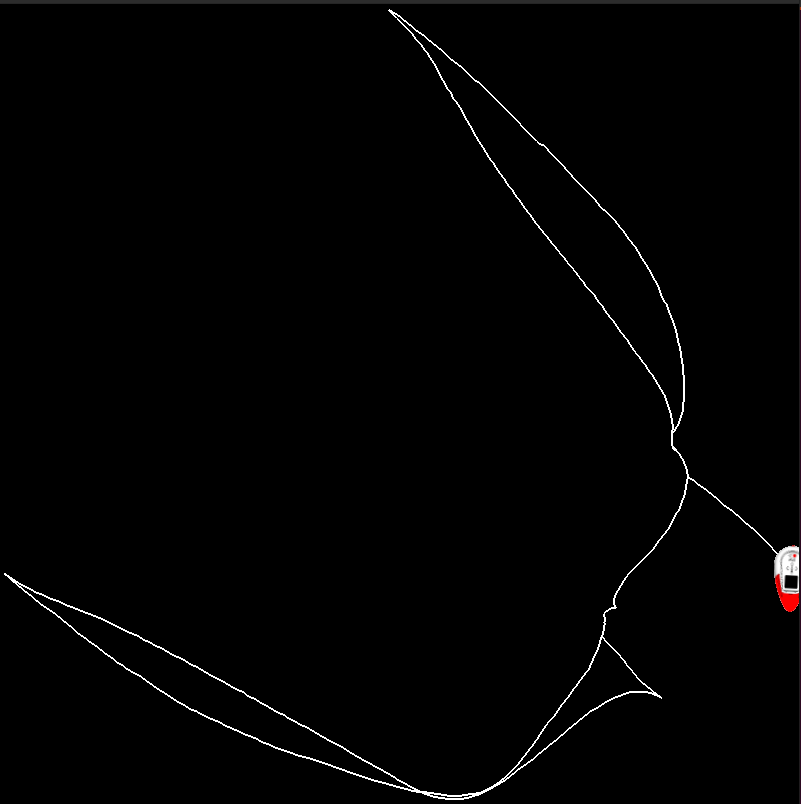
\includegraphics[height=0.3\textheight]{hospital-1stStage.png}\label{fig:mapsHospital1st}}
    \hfill
    \subfloat[Both stages approaches]{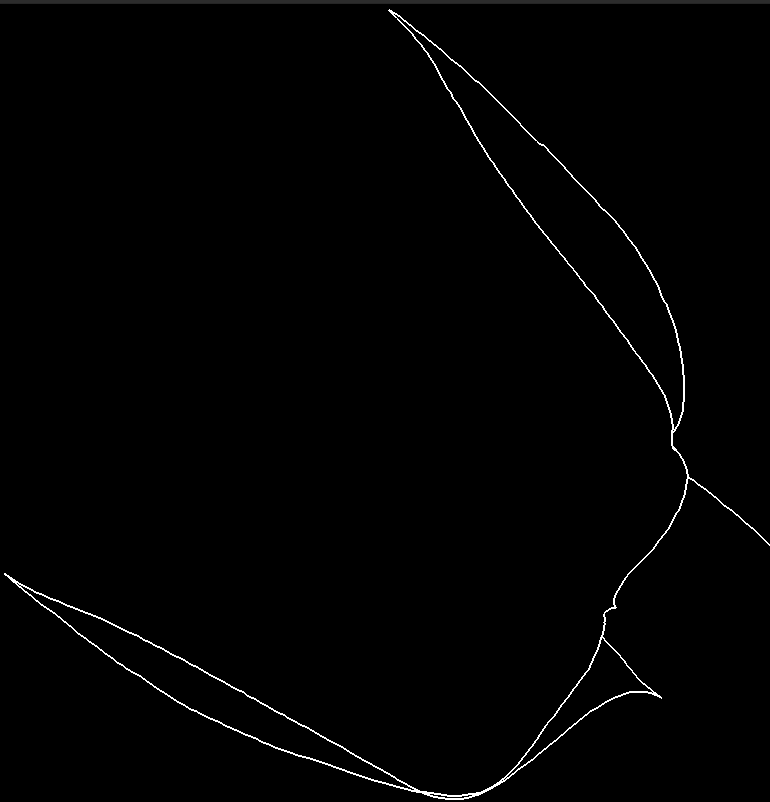
\includegraphics[height=0.3\textheight]{hospital-bothStages.png}\label{fig:mapsHospitalBot}}
    \\
    \subfloat[OpenRatSLAM]{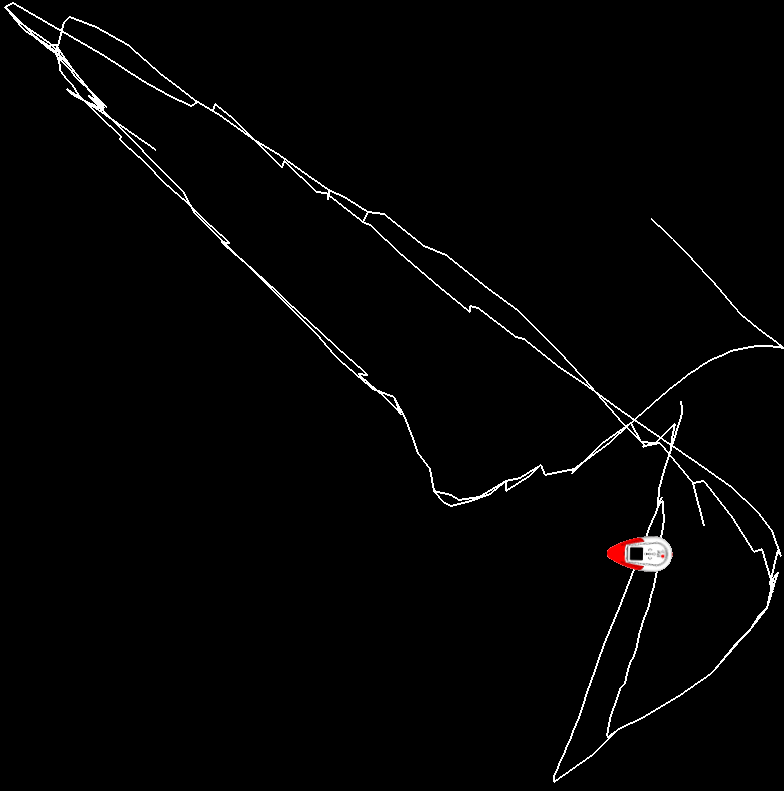
\includegraphics[height=0.3\textheight]{hospital-ratslam.png}\label{fig:mapsHospitalRat}}
    \hfill
    \subfloat[Exact trajectory]{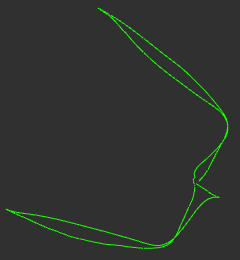
\includegraphics[height=0.3\textheight]{hospital-exact.png}\label{fig:mapsHospitalEx}}
    \caption{Generated experience maps in the hospital environment}
    \label{fig:mapsHospital}
\end{figure}

Figures \ref{fig:mapsWarehouse}, \ref{fig:mapsHouse}, and \ref{fig:mapsHospital} show the generated experience maps by every approach, including the OpenRatSLAM, together with the exact trajectory. The pictures clearly show that the results generated by the approaches with only the first stage and with both stages are almost identical. Even if the accuracy of the 2-stage approach was slightly better, the difference was too small to influence the results of the RatSLAM algorithm significantly. However, after comparing the generated maps with the exact trajectory, we can see that the results are satisfactory and that the suggested approaches are fully compatible with the RatSLAM algorithm.\par
Furthermore, the results from the hospital environment presented in Figure \ref{fig:mapsHospital} clearly show that the suggested approaches can outperform the OpenRatSLAM even in the generated trajectories. Because of the symmetry of the environment, the false evaluations of the visual scene recognition approach influenced the generated trajectory so significantly that it was entirely different from the exact one, and therefore, the OpenRatSLAM algorithm completely failed. However, the LiDAR sensors are considerably more precise in object distance estimation than a camera image, so the symmetry of the environment did not cause so many problems, and the generated results from the approaches suggested in this thesis were satisfactory.

\section{Discussion}\label{section:Discussion}
